% PVLDB Vol. 20 投稿精修版主文件（严格 12 页正文上限，不含参考文献，无附录；已预留 0.5 页总览图余量）
% 注意：acmart 已内置加载 newtxmath、xcolor 与 hyperref，请勿重复加载 amssymb 以免 \Bbbk 冲突

\documentclass[sigconf, nonacm, balance=false]{acmart}

\usepackage{amsmath,amsthm}
\usepackage{booktabs,array,multirow,tabularx}
\usepackage{algorithm}
\usepackage{algpseudocode}
\usepackage{subcaption}
\usepackage{microtype}

% 定理、引理、命题与定义环境
\newtheorem{theorem}{Theorem}
\newtheorem{proposition}[theorem]{Proposition}
\newtheorem{lemma}[theorem]{Lemma}
\newtheorem{corollary}[theorem]{Corollary}
\theoremstyle{definition}
\newtheorem{definition}{Definition}

% 排版容差与浮动体紧凑控制，防止双栏窄行公式溢出或跨栏图表留白
\tolerance=1500
\emergencystretch=2em
\widowpenalty=10000
\clubpenalty=10000
\setlength{\textfloatsep}{6pt plus 1.5pt minus 1.5pt}
\setlength{\floatsep}{5pt plus 1.5pt minus 1.5pt}
\setlength{\dbltextfloatsep}{6pt plus 1.5pt minus 1.5pt}
\setlength{\dblfloatsep}{5pt plus 1.5pt minus 1.5pt}
\captionsetup{skip=3pt}
\graphicspath{{figures/}{../vldb/figures/}}

% 常用数学符号与系统名称宏定义
\newcommand{\rquiver}{Pelorus}
\newcommand{\pelorus}{Pelorus}
\newcommand{\quiver}{QuIVer}
\newcommand{\Bball}{\mathbb{B}_c^D}
\newcommand{\Bunit}{\mathbb{B}_1^D}
\newcommand{\Lmod}{\mathbb{L}_c^D}
\newcommand{\Sunit}{\mathbb{S}^{D-1}}
\newcommand{\R}{\mathbb{R}}
\newcommand{\E}{\mathbb{E}}
\newcommand{\Var}{\operatorname{Var}}
\newcommand{\Cov}{\operatorname{Cov}}
\newcommand{\MNR}{\mathrm{MNR}}
\newcommand{\sgn}{\operatorname{sgn}}
\newcommand{\arccosh}{\operatorname{arccosh}}
\newcommand{\atanh}{\operatorname{atanh}}
\newcommand{\asinh}{\operatorname{asinh}}
\newcommand{\popcnt}{\operatorname{popcnt}}
\newcommand{\missing}{\textemdash}
\DeclareMathOperator*{\argmin}{arg\,min}
\DeclareMathOperator*{\argmax}{arg\,max}

% PVLDB Vol. 20 元数据配置（单盲投稿）
\newcommand\vldbdoi{XX.XX/XXX.XX}
\newcommand\vldbpages{XXX-XXX}
\newcommand\vldbvolume{20}
\newcommand\vldbissue{1}
\newcommand\vldbyear{2027}
\newcommand\vldbauthors{\authors}
\newcommand\vldbtitle{\shorttitle}
\newcommand\vldbavailabilityurl{https://github.com/Astrmira/Pelorus}
\newcommand\vldbpagestyle{plain}

\begin{document}

\title[Pelorus: Warped-Product Graph Indexing for Hyperbolic Vector Search]{Pelorus: Warped-Product Graph Indexing for Hyperbolic Vector Search}

\author{Wenxuan Xiao}
\affiliation{%
  \institution{Astrmira Tech.}
  \country{China}
}
\email{w.xiao@astrmira.com}

\author{Xu Cao}
\affiliation{%
  \institution{Astrmira Tech.}
  \country{China}
}
\email{x.cao@astrmira.com}

\begin{abstract}
% 论文摘要（精修投稿版，约 160 词）：聚焦研究问题、负曲率几何障碍、翘曲乘积极坐标设计与实测结论
Hyperbolic embeddings in the {Poincar\'e} ball and {Lorentz} hyperboloid capture hierarchies with low distortion, yet million-scale approximate nearest neighbor ({ANN}) search faces a fidelity--memory dilemma: flat inner-product proxies distort geodesic order across radial shells, whereas native hyperbolic graphs fetch full-precision vectors per hop or quantize ambient coordinates without conformal decoupling.
Transplanting flat {Vamana} pruning and low-bit codes also fails because inward-bending geodesics let interior hubs occlude spherical neighborhoods, conformal weights $(1 - c\|x\|_2^2)^{-1}$ break cross-shell query-noise cancellation, and tight boundary cones suffer margin-to-noise ratio ({$\MNR$}) collapse.

We present \textbf{\rquiver{}}, an in-memory warped-product graph index pairing a 32-byte unquantized FP32 radial/conformal header with scale-invariant 2-bit Sign-Magnitude ({SM}) spherical bitplanes and tail FP64 reranking.
\rquiver{} attenuates intra-cluster tangent error via purity-gated zero-byte-per-vertex tangent-cone residuals, builds fiber-bundle graphs via inside-out \emph{QuadriPrune} and degree-preserving chord swaps (achieving full entry reachability across all measured graphs), and co-locates headers, stabilized 256-bit sketches, and bitplanes in $4096$\,B pages scored by a 3-to-2 carry-save {AVX2} kernel and orthogonal-projection refinement.

Across eight {AMD Zen~4} benchmarks, \rquiver{} accelerates {Cohere-1M} builds by $5.44\times$ and cuts hot memory by $2.60\times$ versus 8-bit polar codes, lifts {Cohere-1M} $99\%$-recall QPS by $4.30\times$/$6.31\times$ (1T/24T), reaches $53{,}483$\,QPS on {MERU-1M} ($3.37\times$--$3.88\times$ over {HyperspaceDB} FP32), and raises {Clustered-Narrow} recall from $34.22\%$ to $99.385\%$ at $L=256$ ($99.80\%$ at $L=384$; $1.84\times$--$4.56\times$ over {HyperspaceDB}), while characterizing a configuration-dependent recall trade-off on isotropic narrow shells.

\end{abstract}

\maketitle

% PVLDB 官方格式声明块
\pagestyle{\vldbpagestyle}
\begingroup\small\noindent\raggedright\textbf{PVLDB Reference Format:}\\
\vldbauthors. \vldbtitle. PVLDB, \vldbvolume(\vldbissue): \vldbpages, \vldbyear.\\
\href{https://doi.org/\vldbdoi}{doi:\vldbdoi}
\endgroup
\begingroup
\renewcommand\thefootnote{}\footnote{\noindent
This work is licensed under the Creative Commons BY-NC-ND 4.0 International License. Visit \url{https://creativecommons.org/licenses/by-nc-nd/4.0/} to view a copy of this license. For any use beyond those covered by this license, obtain permission by emailing \href{mailto:info@vldb.org}{info@vldb.org}. Copyright is held by the owner/author(s). Publication rights licensed to the VLDB Endowment. \\
\raggedright Proceedings of the VLDB Endowment, Vol. \vldbvolume, No. \vldbissue\ %
ISSN 2150-8097. \\
\href{https://doi.org/\vldbdoi}{doi:\vldbdoi} \\
}\addtocounter{footnote}{-1}\endgroup

\ifdefempty{\vldbavailabilityurl}{}{
\vspace{.2cm}
\begingroup\small\noindent\raggedright\textbf{PVLDB Artifact Availability:}\\
The source code, data, and/or other artifacts have been made available at \url{\vldbavailabilityurl}.
\endgroup
}

% 正文模块化章节（严格控制在 11.5 页内，预留 0.5 页供架构总览图挂载）
% 第一章：引言（精修投稿版，已预留约 0.5 页架构总览图空间）
\section{Introduction}
\label{sec:intro}

Embedding text, images, and structured entities into negatively curved {Riemannian} manifolds---the {Poincar\'e} ball $\Bball$ and {Lorentz} hyperboloid $\Lmod$---captures trees, ontologies, and asymmetric entailment cones with exponentially lower distortion than flat {Euclidean} spaces~\cite{nickel2017poincare,sala2018representation,ganea2018entailment,gu2019mixed}.
Modern encoders scale curved representations across graph neural networks~\cite{nickel2018lorentz,chami2019hgcn}, hyperbolic Transformers and vision backbones~\cite{chen2022fully,khrulkov2020hyperbolic,ermolov2022hyperbolic}, million-scale vision-language alignment ({MERU}~\cite{desai2023meru}), and retrieval-augmented generation ({HypRAG}~\cite{madhu2026hyprag,lewis2020rag}).

Serving low-latency, high-recall approximate nearest neighbor ({ANN}) search over curved manifolds remains a systems bottleneck.
In flat spaces, proximity graphs ({HNSW}~\cite{malkov2020hnsw}, {NSG}~\cite{fu2019nsg}, {Vamana}/{DiskANN}~\cite{subramanya2019diskann,azizi2025graph}) paired with compact in-memory codes ({LVQ}~\cite{aguerrebere2023similarity}, {BBQ}~\cite{trent2024bbq}, {SymphonyQG}~\cite{gou2025symphonyqg}, and 2-bit Sign-Magnitude ({SM}) in {\quiver}~\cite{xiao2026quiver}) restrict cold FP32 vector reads to tail reranking.
In hyperbolic space, existing choices force a costly trade-off: hyperbolic {LSH}~\cite{deng2026hyperboliclsh} requires wide multi-table probing at $99\%+$ recall, flattening curved manifolds into inner-product proxies in {Faiss}~\cite{johnson2019billion,douze2024faiss}, {Milvus}~\cite{wang2021milvus}, {AnalyticDB-V}~\cite{wei2020analyticdb}, or {VBASE}~\cite{zhang2023vbase} conflates radial depth with angular similarity, and native hyperbolic graphs ({NMSLIB}~\cite{boytsov2013engineering}, Prokhorenkova et al.~\cite{prokhorenkova2022hyperbolic}, {HyperspaceDB}~\cite{glukhota2026hyperspacedb}) traverse exact vectors ($2\text{--}6$\,KB per hop with FP64 near $\|x\|_2 \to 1/\sqrt{c}$) or apply unfactored ambient quantization under single-predicate pruning.

\subsection{Why Flat Graph Indexing Breaks Under Negative Curvature}
\label{subsec:intro_obstructions}

Geometrically, $\Bball$ is a \emph{warped product} $\R_{\ge 0} \times_{\frac{1}{\sqrt{c}}\sinh(\sqrt{c}R)} \Sunit$ coupling radial depth $R$ with an exponentially expanding sphere.
Transplanting flat {Vamana} pruning~\cite{subramanya2019diskann} or flat compressed traversal~\cite{aguerrebere2023similarity,gao2024rabitq,xiao2026quiver} onto $\Bball$ fails due to three coupled obstructions:
\begin{enumerate}
  \item \textbf{Cross-Shell Non-Cancellation and Lorentz Blowup.}
  In flat cosine ranking, shared query quantization noise cancels as $u_x \to u_y$~\cite{xiao2026decisions}.
  In $\Bball$, directional inner products are weighted by $W(r_q, r_v) = \frac{2}{c}\sinh\rho_q\sinh\rho_v$: whenever $r_x \ne r_y$, query error leaves an uncancelled residual proportional to $W(r_q, r_y) - W(r_q, r_x)$, while directly quantizing $(D+1)$-D {Lorentz} spatial coordinates scales noise by $\|\tilde{z}\|_2 = \Theta(e^\rho)$.

  \item \textbf{Radial Occlusion and Same-Shell Cone Collapse.}
  Because geodesics bend toward $0 \in \Bball$, an interior neighbor $p$ ($R_p < R_u$) admitted during {Vamana} pruning~\cite{subramanya2019diskann} occludes \emph{every} candidate inside $R_v \le (R_u - \alpha R_p)/(\alpha + 1)$ across all angles $\theta_{pv} \in [0, \pi]$, while along an outer shell $\rho = \sqrt{c}R$, negative curvature contracts the unoccluded angular cone against $p = 0$ exponentially as $\sin(\theta_{uv}/2) < \sinh(\frac{\alpha}{2}\rho)/\sinh\rho \sim e^{-(2-\alpha)\rho/2}$ ($73.7^\circ$ flat $\to 23.1^\circ$ at $\rho = 4$ for $\alpha = 1.2$).
  On {Cohere-1M}, isotropic pruning strands $518\text{--}626$ boundary islands and cuts $99\%$-recall QPS by $5.26\times$ ($2{,}071 \to 394$).

  \item \textbf{Boundary Cluster Margins and Fixed-Budget Pool Dilution.}
  For equal-depth candidates in a tight cone ($\alpha_v = \langle u_v, \mu_c\rangle \to 1$), the ranking margin scales as $\beta_{q,c}\beta_v$ times the tangent-direction difference, while global-code comparison error depends on candidate-error covariance (Theorem~\ref{thm:tangent_cone}).
  As {$\MNR$} collapses, widening beam $L$ at fixed rerank budget $B$ floods the pool with intra-cluster distractors: on {Clustered-Narrow}, raising $L$ from $256$ to $2{,}048$ lowers recall monotonically from $34.22\%$ to $27.80\%$. Local tangent encoding allocates existing bitplanes to normalized within-cone variation without global rotations~\cite{gao2024rabitq,ge2013opq}, retaining native coordinates outside selected cones~\cite{xiao2026decisions}.
\end{enumerate}

\subsection{Warped-Product Co-Design in \rquiver{}}
\label{subsec:intro_solution}

% 几何与执行总览图分别位于第三章与第四章开头。

We introduce \textbf{\rquiver{}}, a hyperbolic proximity-graph index built on \emph{warped-product polar decoupling}.
Each vector is factored into unquantized FP32 radial scalars $(r_x, F_x, \rho_x)$ ($F_x = f_x/2$) in a 32-byte header and a scale-invariant 2-bit {SM} code on $\Sunit$, keeping directional-code error out of $1 - c r_x^2$.
Every design mechanism is paired directly with its geometric derivation (\S\ref{sec:design}--\S\ref{sec:system}), with full proofs in the supplemental material:
\begin{itemize}
  \item \textbf{Polar Representation and Tangent-Cone Recovery (\S\ref{subsec:polar_layout}--\S\ref{subsec:tangent_cone}):}
  Building on flat comparison-decision theory~\cite{xiao2026decisions}, we prove query depth invariance on isobathic shells, characterize cross-shell query-noise non-cancellation and {Lorentz}-MIPS blowup, and introduce purity-gated zero-byte-per-vertex tangent-cone residuals (\texttt{ResidualConeDict}) that attenuate intra-cone error without global rotations while keeping diffuse manifolds on the zero-overhead global path.

  \item \textbf{Fiber-Bundle Topology and Routing (\S\ref{subsec:compass}--\S\ref{subsec:router}):}
  We establish radial occlusion and exponential cone contraction, motivating inside-out depth seeding, four-channel \emph{QuadriPrune} (stem-excess fibers, shielded rings, and radial elevators), spanning-tree chord-swap repair ($1{,}000{,}000/1{,}000{,}000$ directed {BFS} reachability from entry hubs across all measured graphs), and constrained radial-minimizer routing.

  \item \textbf{Page-Co-Located Execution (\S\ref{sec:system}):}
  We co-locate headers, variance-stabilized 256-bit sketches, and 2-bit bitplanes inside $4096$\,B OS pages (\texttt{HotSmPage}) to avoid secondary {DTLB} walks, pair a 3-to-2 carry-save {AVX2} kernel with deterministic orthogonal-projection pool refinement (\textsc{Stage-0.5}) and Conformal Jacobian plateau gating (\textsc{CJ-Gate}), and rerank in FP64 {SIMD}.

  \item \textbf{Zen~4 Evaluation (\S\ref{sec:eval}):}
  Across eight benchmarks, \rquiver{} speeds up {Cohere-1M} builds by $5.44\times$ over {Polar-FP32} ($1.91\times$ over {Polar-SQ8}), shrinks hot navigation memory to $517.0$\,MB page-co-located ($2.44\times$ below {Polar-SQ8}; $485.0$\,MB / $2.60\times$ split), improves {Cohere-1M} $99\%$-recall QPS by $4.30\times$/$6.31\times$ over {Polar-FP32} ($17.0\times$--$28.3\times$ over {HyperspaceDB} at $95\%$ and $22.9\times$--$58.2\times$ over {Faiss}/{Milvus} at $98\%$), hits $53{,}483$\,QPS on {MERU-1M} ($3.37\times$--$3.88\times$ over {HyperspaceDB} FP32), raises {Clustered-Narrow} recall from $34.22\%$ to $99.385\%$ at $L=256$ ($99.80\%$ at $L=384$), and characterizes recall limits on {Uniform-Narrow}.
\end{itemize}

% 第二章：预备知识与问题形式化（精修投稿版）
\section{Preliminaries and Problem Formulation}
\label{sec:prelim}

\subsection{Hyperbolic Models and Polar Geodesic Proxy}
\label{subsec:models}

For constant negative sectional curvature $-c < 0$, the $D$-dimensional {Poincar\'e} ball is $\Bball = \{x \in \R^D : c\|x\|_2^2 < 1\}$ with conformal metric $g_x^{\mathbb{B}} = f_x^2 I_D$, $f_x = \frac{2}{1 - c\|x\|_2^2}$, and geodesic distance $d_{\mathbb{B}}(q, v) = \frac{1}{\sqrt{c}}\arccosh\bigl(1 + \frac{2c\|q - v\|_2^2}{(1 - c\|q\|_2^2)(1 - c\|v\|_2^2)}\bigr)$.
Encoders such as fully hyperbolic networks~\cite{chen2022fully}, {MERU}~\cite{desai2023meru}, and {HypRAG}~\cite{madhu2026hyprag} output points on the $(D+1)$-D {Lorentz} sheet $\Lmod = \{z = (z_0, \tilde{z}) \in \R \times \R^D : -z_0^2 + \|\tilde{z}\|_2^2 = -1/c,\; z_0 > 0\}$ under $d_{\mathbb{L}}(z, z') = \frac{1}{\sqrt{c}}\arccosh(c(z_0 z'_0 - \langle \tilde{z}, \tilde{z}'\rangle))$.
Stereographic projection
\begin{equation}
  \Pi(z_0, \tilde{z}) = \frac{\tilde{z}}{1 + \sqrt{c}\,z_0} \in \Bball
  \label{eq:lorentz_isometry}
\end{equation}
is an exact isometry ($d_{\mathbb{B}}(\Pi(z), \Pi(z')) = d_{\mathbb{L}}(z, z')$)~\cite{nickel2018lorentz} that drops $z_0$ at ingestion.

Writing $x = r_x u_x$ with radius $r_x = \|x\|_2 \in [0, 1/\sqrt{c})$, direction $u_x \in \Sunit$ ($u_0 = e_1$), geodesic radius $R_x = d_{\mathbb{B}}(0, x)$, and depth $\rho_x = \sqrt{c}\,R_x = 2\atanh(\sqrt{c}\,r_x)$ ($\sinh\rho_x = \sqrt{c}\,r_x f_x$, $\cosh\rho_x = f_x - 1$) identifies $\Bball \setminus \{0\}$ with the warped product $(0, \infty) \times_{\frac{1}{\sqrt{c}}\sinh(\sqrt{c}R)} \Sunit$ under $\mathrm{d}s^2 = \mathrm{d}R^2 + \frac{1}{c}\sinh^2(\sqrt{c}R)\,\mathrm{d}\Omega_{D-1}^2$.
For cosine $\gamma_{qv} = \langle u_q, u_v\rangle = \cos\theta_{qv} \in [-1, 1]$, expanding $\|q - v\|_2^2 = (r_q - r_v)^2 + 2 r_q r_v(1 - \gamma_{qv})$ gives the \emph{polar geodesic proxy}
\begin{equation}
  P_{\mathbb{B}}(q, v) \triangleq \|q - v\|_2^2 f_q f_v = R(r_q, r_v) + W(r_q, r_v)\bigl(1 - \gamma_{qv}\bigr),
  \label{eq:polar_proxy}
\end{equation}
where $R(r_q, r_v) = (r_q - r_v)^2 f_q f_v$ and $W(r_q, r_v) = 2 r_q r_v f_q f_v = \frac{2}{c}\sinh\rho_q\sinh\rho_v$.
By the hyperbolic law of cosines, $\frac{c}{4}P_{\mathbb{B}}(q, v) = \sinh^2\bigl(\frac{\sqrt{c}}{2}d_{\mathbb{B}}(q, v)\bigr)$, so
\begin{equation}
  \begin{aligned}
    d_{\mathbb{B}}(q,v)
    &=\frac{1}{\sqrt c}\arccosh\!\left(1+\frac c2 P_{\mathbb B}(q,v)\right)\\
    &=\frac{2}{\sqrt c}\asinh\!\left(\frac12\sqrt{cP_{\mathbb B}(q,v)}\right).
  \end{aligned}
  \label{eq:proxy_to_geodesic}
\end{equation}
Strict monotonicity of~\eqref{eq:proxy_to_geodesic} makes $P_{\mathbb{B}}$ order-isomorphic to $d_{\mathbb{B}}$, deferring $\asinh$ to the final $k$ results.
The implementation stores $F_v = f_v/2 = (1 - c r_v^2)^{-1}$ and evaluates $P_{\mathrm{impl}} = P_{\mathbb{B}}/4$ with $d_{\mathbb{B}} = \frac{2}{\sqrt{c}}\asinh(\sqrt{c\,P_{\mathrm{impl}}})$ across beam thresholds, radial gates, and Jacobian scales (as $c \to 0^+$, $P_{\mathrm{impl}}(q, v) \to \|q - v\|_2^2$).

\subsection{Two-Level Spherical SM and Comparison Operators}
\label{subsec:sm_decisions}

Following {\quiver}'s training-free 2-bit {SM} bitplane encoding~\cite{xiao2026quiver}---whose conditional-mean Pythagorean identity (Lemma~\ref{lem:sm_pythagorean}) underpins our orthogonal-projection refinement (\S\ref{sec:system})---$u_v \in \Sunit$ is encoded into sign bitplane $s_{v,i} = \mathbb{I}[u_{v,i} \ge 0]$ and strong-magnitude bitplane $m_{v,i} = \mathbb{I}[|u_{v,i}| > \tau_v]$ ($\tau_v = \frac{1}{D}\sum_{j=1}^D |u_{v,j}|$, strong count $s_v = \sum_{i=1}^D m_{v,i}$).
Partitioning coordinates into $I_{0,v} = \{i : m_{v,i} = 0\}$ and $I_{1,v} = \{i : m_{v,i} = 1\}$ defines conditional means $a_v = \frac{1}{D - s_v}\sum_{i \in I_{0,v}} |u_{v,i}|$ ($0$ if $s_v = D$), $b_v = \frac{1}{s_v}\sum_{i \in I_{1,v}} |u_{v,i}|$ ($0$ if $s_v = 0$), and step $\delta_v = b_v - a_v$ ($\delta_v \ge 0$ for $0 < s_v < D$; at $s_v = 0$, $b_v = 0$ gives $\delta_v = -a_v$ so all reconstructed coordinates use $a_v$).

\begin{lemma}[Deterministic Two-Level {SM} Pythagorean Identity]
\label{lem:sm_pythagorean}
For any $u_v \in \Sunit$, the conditional-mean code $\hat{u}_{v,i} = \sgn(u_{v,i})(a_v + \delta_v m_{v,i})$ ($\sgn(0) = +1$) uniquely minimizes $\|u_v - \tilde{u}\|_2^2$ over two-level vectors sharing $(s_v, m_v)$ with unique populated-group means and zero distributional assumptions, satisfying
\begin{equation}
  \langle u_v, \hat{u}_v\rangle = (D - s_v)a_v^2 + s_v b_v^2 = \|\hat{u}_v\|_2^2 \triangleq \sigma_v^2 \in (0, 1],
  \label{eq:sm_pythagorean}
\end{equation}
and $\|u_v - \hat{u}_v\|_2^2 = 1 - \sigma_v^2$.
For $\bar{x} = \neg(s_q \oplus s_v)$, five popcounts $p_{\oplus} = \popcnt(\bar{x})$, $p_{10} = \popcnt(\bar{x} \wedge m_q)$, $p_{01} = \popcnt(\bar{x} \wedge m_v)$, $p_{11} = \popcnt(\bar{x} \wedge m_q \wedge m_v)$, and $n_{11} = \popcnt(m_q \wedge m_v)$ evaluate $\langle \hat{u}_q, \hat{u}_v\rangle = a_q a_v(2 p_{\oplus} - D) + a_q\delta_v(2 p_{01} - s_v) + \delta_q a_v(2 p_{10} - s_q) + \delta_q\delta_v(2 p_{11} - n_{11})$ exactly (proved in the supplemental material).
\end{lemma}
\begin{proof}[Proof Sketch]
Splitting $\sum_i |u_{v,i}|(a_v + \delta_v m_{v,i})$ over $I_{0,v}, I_{1,v}$ yields $(D - s_v)a_v^2 + s_v b_v^2 = \|\hat{u}_v\|_2^2$, so $\langle u_v - \hat{u}_v, \hat{u}_v\rangle = 0$.
Expanding $(2\bar{x}_i - 1)$ across $\{1, m_q, m_v, m_q m_v\}$ gives the bilinear form.
\end{proof}

The main hop scorer uses Lemma~\ref{lem:sm_pythagorean}'s five-popcount product with precomputed FP32 norms: for $t = \operatorname{clip}_{[-1,1]}(\langle \hat{u}_q, \hat{u}_v\rangle / (\sigma_q\sigma_v))$ and $\kappa = \operatorname{clip}_{[0.5,1]}(\sigma_q\sigma_v)$, it applies
\begin{equation}
  \hat{\gamma}_{\mathrm{sym}} = \frac{t}{\kappa + (1 - \kappa)t^2},
  \label{eq:sm_calibration}
\end{equation}
while canonical codes $\sgn(u_i)(1 + m_i) \in \{\pm 1, \pm 2\}$ with inverse norm $(D + 3 s_v)^{-1/2}$ supply legacy scoring paths.

\paragraph{Problem Statement and Comparison Operators.}
Given $\mathcal{X} \subset \Bball$ ($|\mathcal{X}| = N$) and query $q \in \Bball$, {ANN} search returns $\widehat{\mathcal{N}}_k(q)$ maximizing $\operatorname{Recall@}k = |\widehat{\mathcal{N}}_k(q) \cap \mathcal{N}_k(q)| / k$ against {QPS} and p99 latency.
By flat comparison-decision stability theory~\cite{xiao2026decisions}, quantized graph indexing depends on sign preservation of two binary operators rather than $|\widehat{P}_{\mathbb{B}} - P_{\mathbb{B}}|$:
(1)~\emph{shared-query ranking} $\Psi_{\mathrm{rank}}(q; x, y) \triangleq P_{\mathbb{B}}(q, x) - P_{\mathbb{B}}(q, y)$ in beam search, and
(2)~\emph{shared-target pruning} $\Psi_{\mathrm{prune}}(u, w, v; \alpha) \triangleq \alpha\,d_{\mathbb{B}}(w, v) - d_{\mathbb{B}}(u, v) \le 0$ ($\alpha > 1$) in {Vamana} construction~\cite{subramanya2019diskann}, whose flip probability under $\widehat{\Psi} = \Psi + \Delta\widehat{\Psi}$ is governed by $\MNR(\widehat{\Psi}) \triangleq |\E[\widehat{\Psi}]| / \sqrt{\Var(\Delta\widehat{\Psi})}$~\cite{xiao2026decisions}.

% 第三章：极坐标共形解耦表示、纤维丛构图与凸支撑路由（合并数学依据与核心算法设计）
\section{Warped-Product Representation, Topology, and Routing}
\label{sec:design}

\begin{figure*}[t]
  \centering
  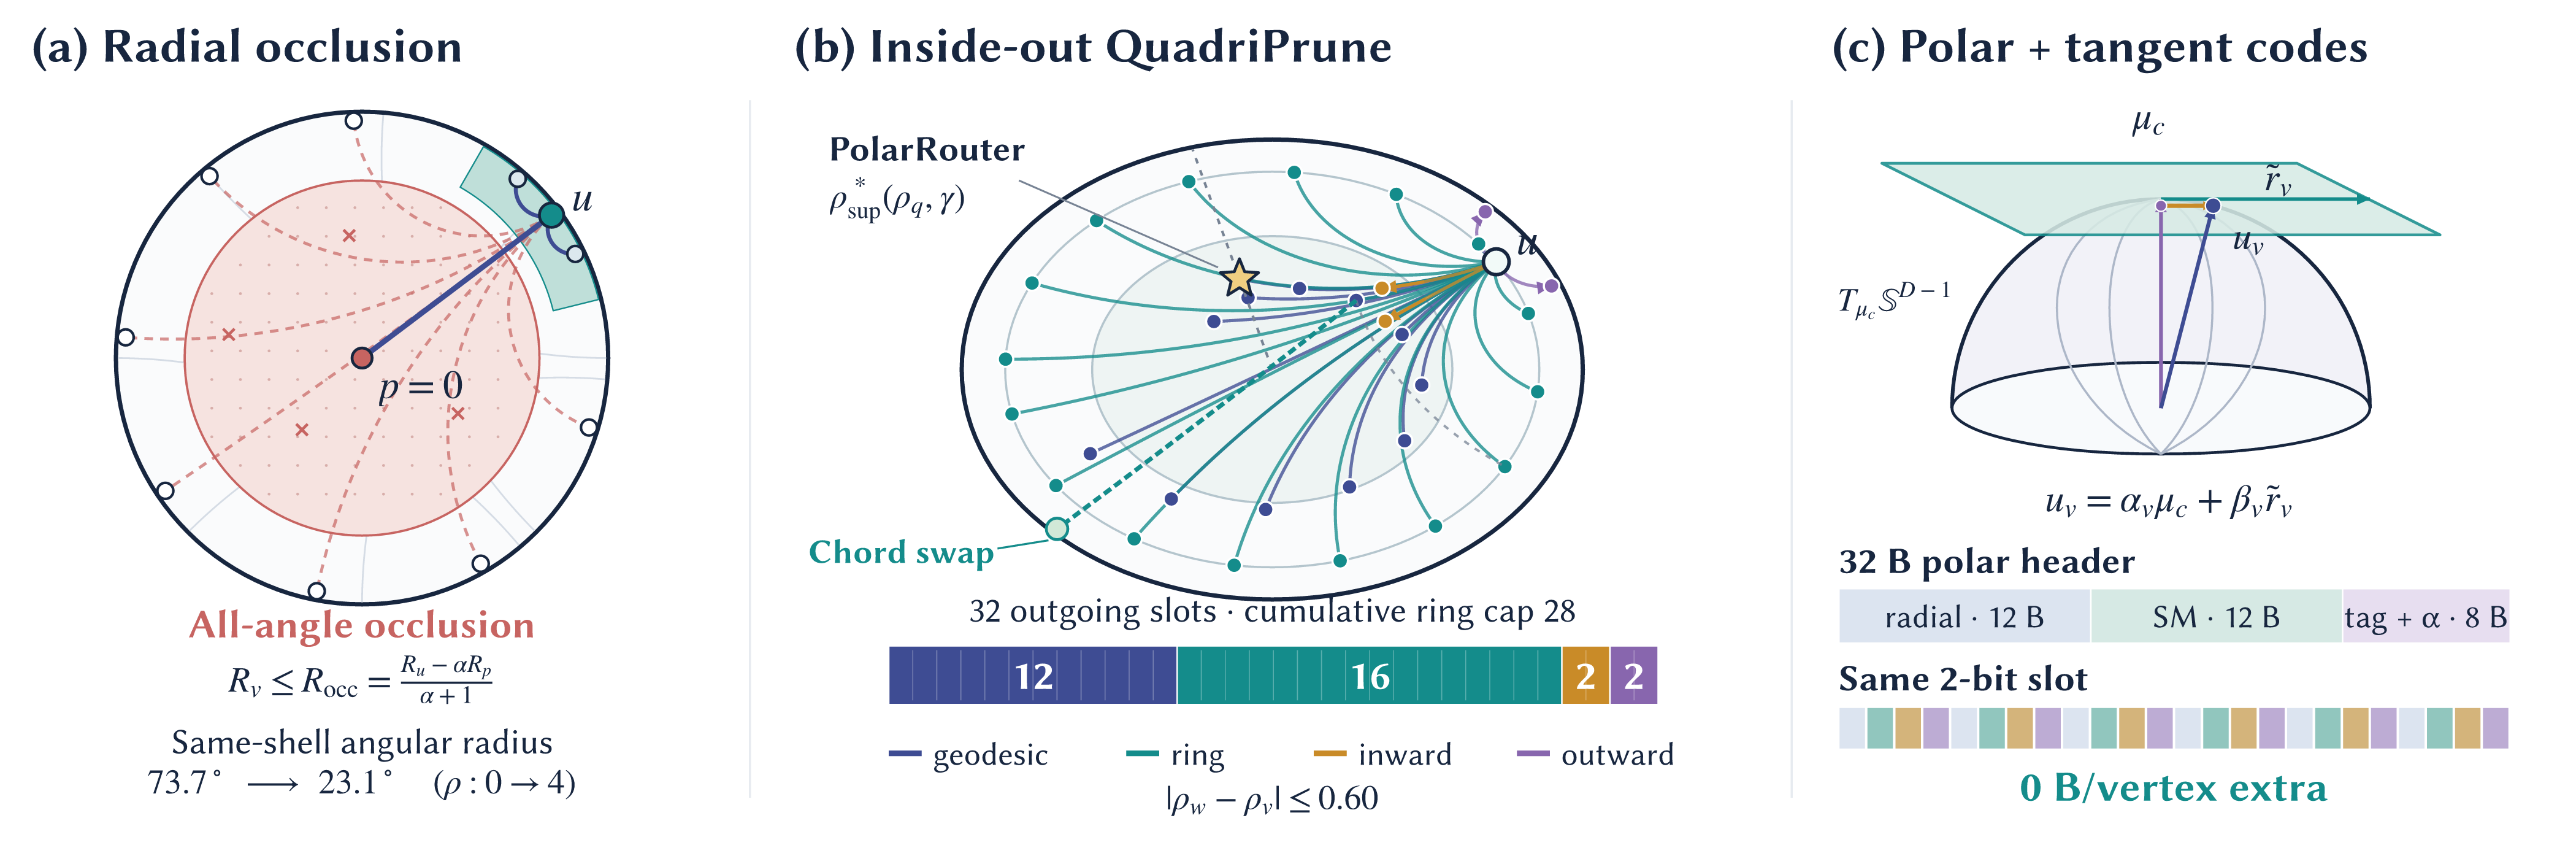
\includegraphics[width=0.95\textwidth]{pelorus_geometry.png}
  \caption{Geometric design of \rquiver{}. (a)~An origin hub exposes all-angle inner-ball occlusion and a shrinking same-shell angular cap ($\alpha=1.2$). (b)~A 32-slot example allocates 12 geodesic, 16 ring, two inward, and two outward links, with a cumulative ring cap of 28. \texttt{PolarRouter} selects ray-support entries, and chord swaps attach islands while preserving the BFS tree. (c)~Tangent encoding reuses the polar header and directional bitplanes, with cosine-error multiplier $\beta_{q,c}\beta_v$. On synthetic {Clustered-Narrow}, Recall@10 rises from $34.22\%$ to $99.385\%$ at $L=256,B=128$.}
  \label{fig:geometry_overview}
\end{figure*}

Figure~\ref{fig:geometry_overview} summarizes the geometry and representation. We co-design \rquiver{}'s representation, topology, and router by pairing each curved-manifold pathology directly with its resolving primitive (complete proofs in the supplemental material).

\subsection{Conformal Flip Analysis and 32-Byte Polar Header}
\label{subsec:polar_layout}

Let $\varepsilon_\angle(q, v) \triangleq \hat{\gamma}(u_q, u_v) - \gamma_{qv}$ be directional error in $\widehat{P}_{\mathbb{B}}(q, v) = R(r_q, r_v) + W(r_q, r_v)(1 - \hat{\gamma}(u_q, u_v))$.
For the uncalibrated bilinear product $\langle \hat{u}_q/\sigma_q, \hat{u}_v/\sigma_v\rangle$ (before calibration in~\eqref{eq:sm_calibration}) with $e_z = \hat{u}_z / \sigma_z - u_z$, bilinear decomposition~\cite{bussgang1952crosscorrelation,xiao2026decisions} gives $\varepsilon_\angle(q, v) = \eta_q(u_v) + \eta_v(u_q) + \xi_{qv}$ ($\eta_q(u_v) = \langle e_q, u_v\rangle$, $\eta_v(u_q) = \langle u_q, e_v\rangle$, $\xi_{qv} = \langle e_q, e_v\rangle$).
In flat cosine search ($W \equiv 1$), $\eta_q(u_x) - \eta_q(u_y) = \langle e_q, u_x - u_y\rangle$ has variance $(u_x - u_y)^\top\Sigma_q(u_x - u_y)$ ($\Sigma_q = \Cov(e_q)$, $\|\Sigma_q\|_2 = O(1/D)$), giving standard deviation $O(\|u_x - u_y\|_2/\sqrt{D})$~\cite{xiao2026decisions}. On $\Bball$,~\eqref{eq:cross_shell_var} models one term before calibration. A hop-score inversion also depends on the true pairwise margin.

\begin{theorem}[Conformal Flip Criterion, Depth Invariance, and Lorentz-MIPS Blowup]
\label{thm:conformal_flip}
Let $q, x, y \in \Bball$ ($r_q > 0$) satisfy $\Delta_P(q; x, y) \triangleq P_{\mathbb{B}}(q, y) - P_{\mathbb{B}}(q, x) > 0$ with real-valued radial scalars $(r_z, f_z)$ (FP32 rounding bounds in the supplemental material). Then:
(1)~\textbf{Query depth invariance:} $\widehat{P}_{\mathbb{B}}(q, y) \le \widehat{P}_{\mathbb{B}}(q, x)$ holds iff $r_y f_y \varepsilon_\angle(q, y) - r_x f_x \varepsilon_\angle(q, x) \ge \Delta_P / (2 r_q f_q)$. On an isobathic shell ($r_x = r_y = r>0$), this reduces to $\varepsilon_\angle(q, y) - \varepsilon_\angle(q, x) \ge \gamma_{qx} - \gamma_{qy}$, independent of both radii at fixed directions and estimates.
(2)~\textbf{Cross-shell non-cancellation:} For arbitrary $\Sigma_q = \Cov(e_q)$ under bilinear error, mismatched weights $d_q = W(r_q, r_y) - W(r_q, r_x)$ leave uncancelled query variance $d_q^2 u_x^\top\Sigma_q u_x$ at $u_x = u_y$. Specializing to $\Sigma_q = \frac{\kappa_q}{D}(I_D - u_q u_q^\top)$ gives
\begin{equation}
  \begin{aligned}
    &\Var_{e_q}\!\bigl(d_q\eta_q(u_x)\mid u_x=u_y\bigr)\\
    &\quad=\frac{4\kappa_q}{c^2D}\sinh^2\rho_q
      \bigl(\sinh\rho_y-\sinh\rho_x\bigr)^2(1-\gamma_{qx}^2),
  \end{aligned}
  \label{eq:cross_shell_var}
\end{equation}
growing as $\Theta(e^{2\rho_q + 2\max(\rho_x,\rho_y)}/D)$ for fixed shell gap and $1 - \gamma_{qx}^2 > 0$, shrinking to $O(\delta_\rho^2 W^2)$ within $|\rho_y - \rho_x| \le \delta_\rho$, and vanishing at $e_q = 0$.
(3)~\textbf{Spatial Lorentz-MIPS scaling:} Under $\Cov(\epsilon_v) = \Theta(\|\tilde{z}_v\|_2^2 / D)I_D$, quantizing $\tilde{z} = \frac{1}{\sqrt{c}}\sinh\rho_z\,u_z \in \R^D$ on $\Lmod$ without polar separation incurs error standard deviation $\Theta(\frac{1}{c\sqrt{D}}\sinh\rho_q\sinh\rho_v)$ even at $\theta_{qv} = 0$.
\end{theorem}
\begin{proof}[Proof Sketch]
Exact $R, W$ give $\widehat{P}_{\mathbb{B}}(q, v) - P_{\mathbb{B}}(q, v) = -2 r_q f_q r_v f_v \varepsilon_\angle(q, v)$, so dividing by $2 r_q f_q > 0$ proves~(1).
Isolating $d_q\eta_q(u_x)$ yields~\eqref{eq:cross_shell_var}, while $\|\tilde{z}_v\|_2 = c^{-1/2}\sinh\rho_v$ scales spatial steps.
\end{proof}

\paragraph{32-Byte \texttt{PolarNodeMeta} Header.}
Guided by Theorem~\ref{thm:conformal_flip}, \rquiver{} projects $\Lmod \to \Bball$ via~\eqref{eq:lorentz_isometry} and pairs 2-bit {SM} bitplanes ($2\lceil D / 64\rceil \times 8$\,B) with a 32-byte header:
(1)~unquantized FP32 radial scalars $(r_v, F_v, \rho_v)$ ($12$\,B, $F_v = (1 - c r_v^2)^{-1} = f_v/2$, computed in FP64),
(2)~FP32 {SM} scalars $(a_v, \delta_v, \sigma_v)$ ($12$\,B) for hop scoring and \textsc{Stage-0.5}, and
(3)~a 32-bit word packing 20-bit $s_v$ and 12-bit $\text{cone\_id}$ (\texttt{0x0FFF} for global {SM}) plus an FP32 slot ($8$\,B) storing $\alpha_v = \langle u_v, \mu_c\rangle$ on cones or $(D + 3 s_v)^{-1/2}$ on global legacy paths.
At $D = 768, M_0 = 32$ (Table~\ref{tab:node_layout}), logical per-vertex navigation state is $384$\,B with \texttt{SymSketch256} ($517.0$\,MB page-co-located, $2.07\times$ below {Polar-SQ8} at $1{,}069.0$\,MB and $6.52\times$ below {Polar-FP32} at $3{,}373.0$\,MB) or $352$\,B without the sketch ($485.0$\,MB split, $2.20\times$ and $6.95\times$ smaller), separating traversal from the $3{,}072.0$\,MB cold FP32 rerank store.

\begin{table}[t]
  \centering
  \caption{Per-vertex logical hot navigation payload and {Cohere-1M} byte reconciliation ($D=768, M_0=32, N=10^6$).}
  \label{tab:node_layout}
  \footnotesize
  \setlength{\tabcolsep}{3.5pt}
  \begin{tabularx}{\linewidth}{@{}>{\raggedright\arraybackslash}Xrrrr@{}}
    \toprule
    & Header/code/edges & Logical & Hot & Total \\
    Representation & B/vertex & B/vertex & MB & MB \\
    \midrule
    Polar-FP32 & 32/3,072/128 & 3,232 & 3,373 & 3,373 \\
    Polar-SQ8 & 32/768/128 & 928 & 1,069 & 4,141 \\
    \rquiver{}-Split & 32/192/128 & 352 & 485 & 3,557 \\
    \textbf{\rquiver{}} & \textbf{64/192/128} & \textbf{384} & \textbf{517} & \textbf{3,589} \\
    \bottomrule
  \end{tabularx}
  \par\smallskip
  {\scriptsize\raggedright The logical payload counts 32 active edges. Fixed-stride adjacency reserves 64 IDs/vertex ($256$\,MB), plus $4$\,MB for degrees and $0.975$\,MB for routing. Page-co-located codes and headers add $256$\,MB. Total includes one $3{,}072$\,MB FP32 vector store, reused for navigation by Polar-FP32. SQ8/FP32 hot counts include $8$\,MB of inverse norms and exclude an unused $192$\,MB 2-bit benchmark allocation. Totals are index-array accounting in decimal MB. Process RSS also includes benchmark and allocator overhead. An active cone dictionary adds $4CD$ bytes ($0$ on this dataset).\par}
\end{table}

\subsection{Boundary Margin Collapse and Purity-Gated \texttt{ResidualConeDict}}
\label{subsec:tangent_cone}

Even when $e_q = 0$, candidate quantization noise persists inside tight boundary cones around unit axis $\mu_c \in \Sunit$.
Decomposing $u_v = \alpha_v\mu_c + \beta_v\tilde{r}_v$ ($\alpha_v = \langle u_v, \mu_c\rangle$, $\beta_v = \sqrt{1 - \alpha_v^2}$, $\tilde{r}_v \in T_{\mu_c}\Sunit \cap \Sunit$) and $u_q = \alpha_{q,c}\mu_c + \beta_{q,c}\tilde{r}_{q,c}$ writes $\gamma_{qv} = \alpha_{q,c}\alpha_v + \beta_{q,c}\beta_v\langle \tilde{r}_{q,c}, \tilde{r}_v\rangle$.

\begin{theorem}[Tangent-Cone Error Propagation and Fixed-Budget Admission]
\label{thm:tangent_cone}
Consider same-shell candidates $x, y$ with weight $W = W(r_q, r) > 0$, common $\alpha = \sqrt{1 - \beta^2}$ ($\beta, \beta_{q,c} > 0$), and $\Delta_{\tilde{r}} = \langle \tilde{r}_{q,c}, \tilde{r}_y - \tilde{r}_x\rangle \ne 0$ under conditional zero-mean errors:
(1)~\textbf{Pairwise margin and covariance:} The true margin is $W\beta_{q,c}\beta|\Delta_{\tilde{r}}|$. For global cosine errors $g_x, g_y$ with $V_g = \Var(g_y) + \Var(g_x) - 2\Cov(g_y, g_x) > 0$, $\MNR_{\mathrm{global}} = \beta_{q,c}\beta|\Delta_{\tilde{r}}| / \sqrt{V_g}$, collapsing as $\sqrt{V_g}/(\beta_{q,c}\beta|\Delta_{\tilde{r}}|) \to \infty$.
(2)~\textbf{Fixed-budget admission under exchangeable ranks:} If the retained pool holds $N_c(L) \ge B$ cone members including $k_c(L)$ true neighbors and all $B$ rerank slots are drawn from them under a conditional uniform rank permutation, expected true-neighbor admission is $k_c(L) B / N_c(L)$, decreasing iff $k_c(L) / N_c(L)$ decreases.
(3)~\textbf{Exact tangent-error attenuation:} With real-valued axial scalars in
\begin{equation}
  \hat{\gamma}_{\mathrm{cone}}(q, v) \triangleq \alpha_{q,c}\alpha_v + \beta_{q,c}\beta_v\,\hat{\gamma}_{\mathrm{asym}}(\tilde{r}_{q,c}, \tilde{r}_v)
  \label{eq:cone_estimator}
\end{equation}
and $e_v = \hat{\gamma}_{\mathrm{asym}}(\tilde{r}_{q,c}, \tilde{r}_v) - \langle \tilde{r}_{q,c}, \tilde{r}_v\rangle$, cosine error equals $\beta_{q,c}\beta_v e_v$ pointwise. For $V_r = \Var(e_y) + \Var(e_x) - 2\Cov(e_y, e_x) > 0$, $\MNR_{\mathrm{cone}} = |\Delta_{\tilde{r}}| / \sqrt{V_r}$ and $\MNR_{\mathrm{cone}} / \MNR_{\mathrm{global}} = \sqrt{V_g} / (\beta_{q,c}\beta\sqrt{V_r})$. Tangent codes improve MNR exactly when $V_g>(\beta_{q,c}\beta)^2 V_r$.
\end{theorem}
\begin{proof}[Proof Sketch]
Axial terms $\alpha_{q,c}\alpha$ cancel in $\Psi_{\mathrm{rank}}$, so $\Var(X - Y) = \Var(X) + \Var(Y) - 2\Cov(X, Y)$ gives $W^2 V_g$ globally and $W^2\beta_{q,c}^2\beta^2 V_r$ under~\eqref{eq:cone_estimator}, while uniform ranks admit each cone member with probability $B / N_c(L)$.
\end{proof}

\rquiver{} adapts residual normalization~\cite{jegou2011pq} to $\Sunit$ as a fail-safe for clustered boundary cones without perturbing diffuse contrastive manifolds~\cite{wang2020understanding,betser2026infonce,xiao2026decisions} via a two-stage build check over $\min(N, 8{,}192)$ non-origin samples:
(1)~shallow distributions ($p_{90}(\rho) < 1.0$) bypass residual encoding immediately because boundary Jacobian amplification is mild;
(2)~otherwise ($p_{90}(\rho) \ge 1.0$), a spherical leader pass ($\tau_{\mathrm{lead}} = 0.91$, $\le 1{,}024$ seeds) and two spherical-mean rounds ($\langle u_s, \mu_c\rangle \ge 0.94$) retain up to $C \le 512$ axes meeting support $\operatorname{clamp}(\lfloor N_{\mathrm{samp}}/1024\rfloor, 3, 12)$ and purity $\bar{\alpha}_c \ge 0.955$, exiting with $0$ cones if no cluster passes purity.
Vertices with $\alpha_v \ge 0.94$ store the 2-bit {SM} code of $\tilde{r}_v$ in the existing bitplane slot and record $\text{cone\_id}$ in the 12-bit header (\textbf{0\,B/vertex} overhead, $\beta_v^2 \le 0.1164$).
Among the eight primary workloads, MERU-1M and WordNet-Hazy exit at the depth check. Cohere-1M, OpenAI-1536 and the two isotropic sets exit at the purity check. Both clustered sets activate 256 cones ($4CD$ bytes or $0.50$\,MiB at $D=512$).

\subsection{Hyperbolic Vamana Pathologies, QuadriPrune, and Chord-Swap Repair}
\label{subsec:compass}

For {Vamana} pruning~\cite{subramanya2019diskann}, triangle inequalities give a sufficient inner-ball bound. The same-shell formula assumes an origin neighbor. On Cohere, $R_{\mathrm{occ}}\le1.01$, below the first-percentile depth of $1.45$. The bound leaves occlusion farther out unresolved.

\begin{theorem}[Radial Occlusion, Cone Contraction, Escape Cap, and Surrogate Bias]
\label{thm:vamana_pathologies}
On $\Bball$ ($-c < 0$) under pruning slack $\alpha > 1$:
(1)~\textbf{Radial occlusion and cone contraction:} If outer vertex $u$ ($R_u > 0$) admits interior neighbor $p$ ($R_p < R_u / \alpha$), then every $v$ inside $R_v \le R_{\mathrm{occ}} \triangleq (R_u - \alpha R_p)/(\alpha + 1)$ satisfies $\alpha\,d_{\mathbb{B}}(p, v) \le d_{\mathbb{B}}(u, v)$ across all $\theta_{pv} \in [0, \pi]$.
Specifically under negative curvature, for $R_u = R_v = R$ ($\rho = \sqrt{c}R$) and $p = 0$ ($\alpha \in (1, 2)$), $\alpha\,d_{\mathbb{B}}(0, v) \le d_{\mathbb{B}}(u, v)$ holds whenever
\begin{equation}
  \sin(\theta_{uv}/2) \ge \sinh(\tfrac{\alpha}{2}\rho)/\sinh(\rho) \sim e^{-(2-\alpha)\rho/2},
  \label{eq:cone_contraction}
\end{equation}
shrinking the unoccluded cone from $73.7^\circ$ ($c \to 0^+$) to $23.1^\circ$ ($\rho = 4$) and $10.4^\circ$ ($\rho = 6$) at $\alpha = 1.2$.
(2)~\textbf{Angular escape condition:} Candidate $v$ satisfies $d_{\mathbb{B}}(q, v) < R_q$ iff $\gamma_{qv} > \gamma_{\mathrm{esc}}(R_q, R_v) \triangleq \tanh(\sqrt{c}R_v / 2)/\tanh(\sqrt{c}R_q)$. Equality gives $d_{\mathbb{B}}(q,v)=R_q$ for positive depths.
(3)~\textbf{Surrogate bias:} Affine surrogates $\hat{d} = a d + b$ ($a > 0$) yield margin $a[d(u, v) - \alpha d(w, v)] + (1 - \alpha)b$ ($b > 0$ under-prunes, $b < 0$ over-prunes). The geodesic test $\alpha d(w,v)\le d(u,v)$ is equivalent to $P_\alpha(P_{\mathbb B}(w,v))\le P_{\mathbb B}(u,v)$, where $P_\alpha(x)=\frac{2}{c}[\cosh(\alpha\arccosh(1+cx/2))-1]$. Since $P_\alpha(x)>\alpha x$ for $x>0$, using $\alpha P_{\mathbb B}(w,v)$ on the left over-prunes.
\end{theorem}
\begin{proof}[Proof Sketch]
Triangle-inequality sufficient bounds $d_{\mathbb{B}}(p, v) \le R_p + R_v$ and $d_{\mathbb{B}}(u, v) \ge R_u - R_v$ give $R_{\mathrm{occ}}$, while $\sinh(\frac{\sqrt{c}}{2}d_{\mathbb{B}}(u, v)) = \sinh\rho\sin(\theta_{uv}/2)$ yields~\eqref{eq:cone_contraction}.
Expanding $\cosh(\sqrt{c}d_{\mathbb{B}}(q, v)) < \cosh\rho_q$ gives $\gamma_{\mathrm{esc}}$, and $\hat{d}(u, v) - \alpha\hat{d}(w, v)$ isolates $(1 - \alpha)b$.
\end{proof}

\begin{algorithm}[t]
\caption{Warped-Product Construction \& Chord-Swap Repair}
\label{alg:compass_build}
\footnotesize
\begin{algorithmic}[1]
\Require Dataset $\mathcal{X} \subset \Bball$, max out-degree $M_0 = 2M$, build beam $L_c$, slack $\alpha > 1$
\Ensure Graph $G = (V, E)$ with maximum degree $M_0$ and measured entry-reachable set $\mathcal{R}$
\State Build \texttt{PolarNodeMeta}, purity-gated \texttt{ResidualConeDict}, 2-bit {SM}, and \texttt{PolarRouter}
\State Sort $\pi = (v_1, \dots, v_N)$ by $\rho_{v_1} \le \dots \le \rho_{v_N}$ with empty adjacency lists
\For{consecutive radial wave $B_t \subset \pi$ ($\le 256$ vertices) ordered inside-out}
  \For{each $u \in B_t$ in parallel}
    \State $\mathcal{C}_u \gets \textsc{PolarBeamSearch}(G, u, L_c)$ using 2-bit proxy $\widehat{P}_{\mathbb{B}}$
    \State Partition $\le M_0$ edges via \textbf{QuadriPrune}: geodesic fiber (cap $\max(1, \lfloor \frac{3}{8}M_0\rfloor)$) via~\eqref{eq:dom_geo}, shielded ring (cumulative cap $\lfloor \frac{7}{8}M_0\rfloor$, $|\rho_w - \rho_v| \le 0.60$), and inward/outward elevators via~\eqref{eq:elevator_obj} plus fallback fill
    \State Add reverse edges $v \to u$ for $v \in N^+(u)$, re-pruning if $\deg^+(v) > M_0$
  \EndFor
\EndFor
\State Final-prune lists to $M_0$, then $(\mathcal{R}, \texttt{parent}) \gets \textsc{DirectedBFSTree}(G, \text{entry\_hub})$
\For{each $u \in \pi$ with $u \notin \mathcal{R}$}
  \State Find reachable $p \in \mathcal{R}$ in $N^+(u)$, hubs, or 256-vertex core prefix with free slot or removable chord (if none exists, \textbf{continue})
  \State Append $p \to u$ if $\deg^+(p) < M_0$, else swap chord $p \to w^\star$ ($\texttt{parent}[w^\star] \ne p \land \deg^-(w^\star) \ge 2$) with $p \to u$
  \State $\texttt{parent}[u] \gets p$, then expand $(\mathcal{R}, \texttt{parent})$ via incremental {BFS} from $u$
\EndFor
\State \Return fixed-stride graph $G$, reachable set $\mathcal{R}$, and $4096$\,B \texttt{HotSmPage} store
\end{algorithmic}
\end{algorithm}

\paragraph{Inside-Out Seeding, QuadriPrune, and Chord-Swap Repair.}
Algorithm~\ref{alg:compass_build} builds full-database router seeds before connecting $\le 256$-vertex inside-out waves across four cumulative channels ($M_0=32$). The channel weights and shell cutoffs are empirical constants held fixed across datasets.
(1)~\emph{Geodesic fiber} ($12$ slots): with $\tilde{d} = \sqrt{c}d_{\mathbb{B}}$, $\ell_\angle(x, y) = 1 - \hat{\gamma}(u_x, u_y)$, $\Delta_{\mathrm{stem}}(u, v, w) = \max(0, |\rho_u - \rho_v| - |\rho_w - \rho_v|)$, and $\tilde{d}_{\mathrm{eff}}(u, v, w) = \max(0, \tilde{d}(u, v) - \Delta_{\mathrm{stem}})$, neighbor $w$ dominates $v$ iff
\begin{equation}
  \bigl[\ell_\angle(w, v) \le \ell_\angle(u, v)\bigr] \;\land\; \bigl[\alpha\,\tilde{d}(w, v) \le \tilde{d}_{\mathrm{eff}}(u, v, w)\bigr],
  \label{eq:dom_geo}
\end{equation}
enforcing the angular guard and rejecting $\alpha|\rho_w - \rho_v| > \tilde{d}_{\mathrm{eff}}$ in $O(1)$ arithmetic.
(2)~\emph{Shielded ring} ($28$ cumulative slots): orders candidates by $\ell_\angle(u, v) + 0.85|\rho_u - \rho_v|$ and limits $\alpha\ell_\angle(w, v) \le \ell_\angle(u, v)$ to $|\rho_w - \rho_v| \le 0.60$. Only neighbors within this depth gap can suppress a ring candidate.
(3)--(4)~\emph{Inward/outward elevators} (splitting remaining $h = M_0 - s$ slots as $\lfloor h/2\rfloor$ inward on $\rho_v < \rho_u - 0.18$ and outward on $\rho_v > \rho_u + 0.18$, with dominators $\rho_w < \rho_u - 0.10$ / $\rho_w > \rho_u + 0.10$): minimize
\begin{equation}
  J_{\mathrm{elev}}(u, v) \triangleq \ell_\angle(u, v) + 0.15\bigl||\rho_v - \rho_u| - 0.65\bigr|,
  \label{eq:elevator_obj}
\end{equation}
followed by diversity fill ($\ell_\angle + 0.25|\rho_u - \rho_v|$, $|\rho_w - \rho_v| \le 1.0$) and ordered fill (with fixed dataset-independent quotas and tolerances; at constant depth, elevator sets are empty and the ring prunes by angle).
The chord-swap pass repairs the $521\text{--}628$ zero-in-degree boundary islands on {Cohere-1M} while preserving tree edges, achieving $1{,}000{,}000 / 1{,}000{,}000$ directed {BFS} reachability from the entry hub ($0$ islands) across all 21 million-scale {Zen~4} graphs in $<0.3$\,s.

\subsection{Ray Strong Convexity and \texttt{PolarRouter}}
\label{subsec:router}

\begin{proposition}[Radial Lower Bound and Constrained Radial Minimizer]
\label{prop:geodesic_apex}
For $q \in \Bball$ at depth $\rho_q$:
(1)~$P_{\mathbb{B}}(q, v) \ge P_{\mathrm{rad}}(r_q, r_v) \triangleq (r_q - r_v)^2 f_q f_v = \frac{2}{c}(\cosh|\rho_q - \rho_v| - 1)$ for all $v \in \Bball$.
(2)~Along a ray $\{v(\rho) : \rho \in \R\}$ of alignment $\gamma = \langle u_q, \mu_a\rangle$, $g_\gamma(\rho) \triangleq \cosh\rho_q\cosh\rho - \gamma\sinh\rho_q\sinh\rho$ satisfies $g_\gamma''(\rho) = g_\gamma(\rho) \ge \cosh(\rho_q - |\rho|) \ge 1$ ($1$-strong convexity on $\R$) and attains its unique minimizer on $[\rho_{\min}, \rho_{\max}] \subset [0, \infty)$ at $\rho_{\mathrm{sup}}^* = \operatorname{clip}_{[\rho_{\min},\rho_{\max}]}(\rho^*)$ where
\begin{equation}
  \rho^*(\rho_q, \gamma) = \atanh\bigl(\tanh\rho_q \cdot \max(\gamma, 0)\bigr),
  \label{eq:geodesic_apex}
\end{equation}
specializing hyperbolic right-triangle projection to bounded radial support.
\end{proposition}
\begin{proof}[Proof Sketch]
$\gamma_{qv} \le 1$ gives~(1). Differentiating twice gives $g_\gamma''(\rho) \ge \cosh(\rho_q - |\rho|) \ge 1$, $g_\gamma'(\rho) = 0$ yields~\eqref{eq:geodesic_apex}, and clamping follows by strict convexity.
\end{proof}

Avoiding origin-medoid traps (Theorem~\ref{thm:vamana_pathologies}(2)), \texttt{PolarRouter} builds $C = \min(N, \operatorname{clamp}(\lfloor N/100\rfloor, 64, 2048))$ Tammes-style {SM} landmarks~\cite{tammes1930origin} ($64$ coarse landmarks with $128$-cone shortlists when $C > 256$, plus $16$ origin hubs) crossed with $8$ quantile shells ($16{,}384$ cells $\times 8$ IDs at $N = 10^6$), seeding shell representatives via $\rho_{\mathrm{sup}}^*(\rho_q, \gamma)$ over sampled positive database depths and scanning fine cones directly when a dimension-scaled isotropy guard detects low coarse alignment (\S\ref{subsec:eval_ablation}). Validation queries can select hubs alone or full routing jointly with $(L,B)$ for each target and thread count.

% 第四章：面向硬件页表与位级并行的极坐标执行引擎（合并非对称投影/CJ-Gate/草图方差命题与系统算子实现）
\section{Hardware-Conscious Polar Execution Engine}
\label{sec:system}

\begin{figure*}[t]
  \centering
  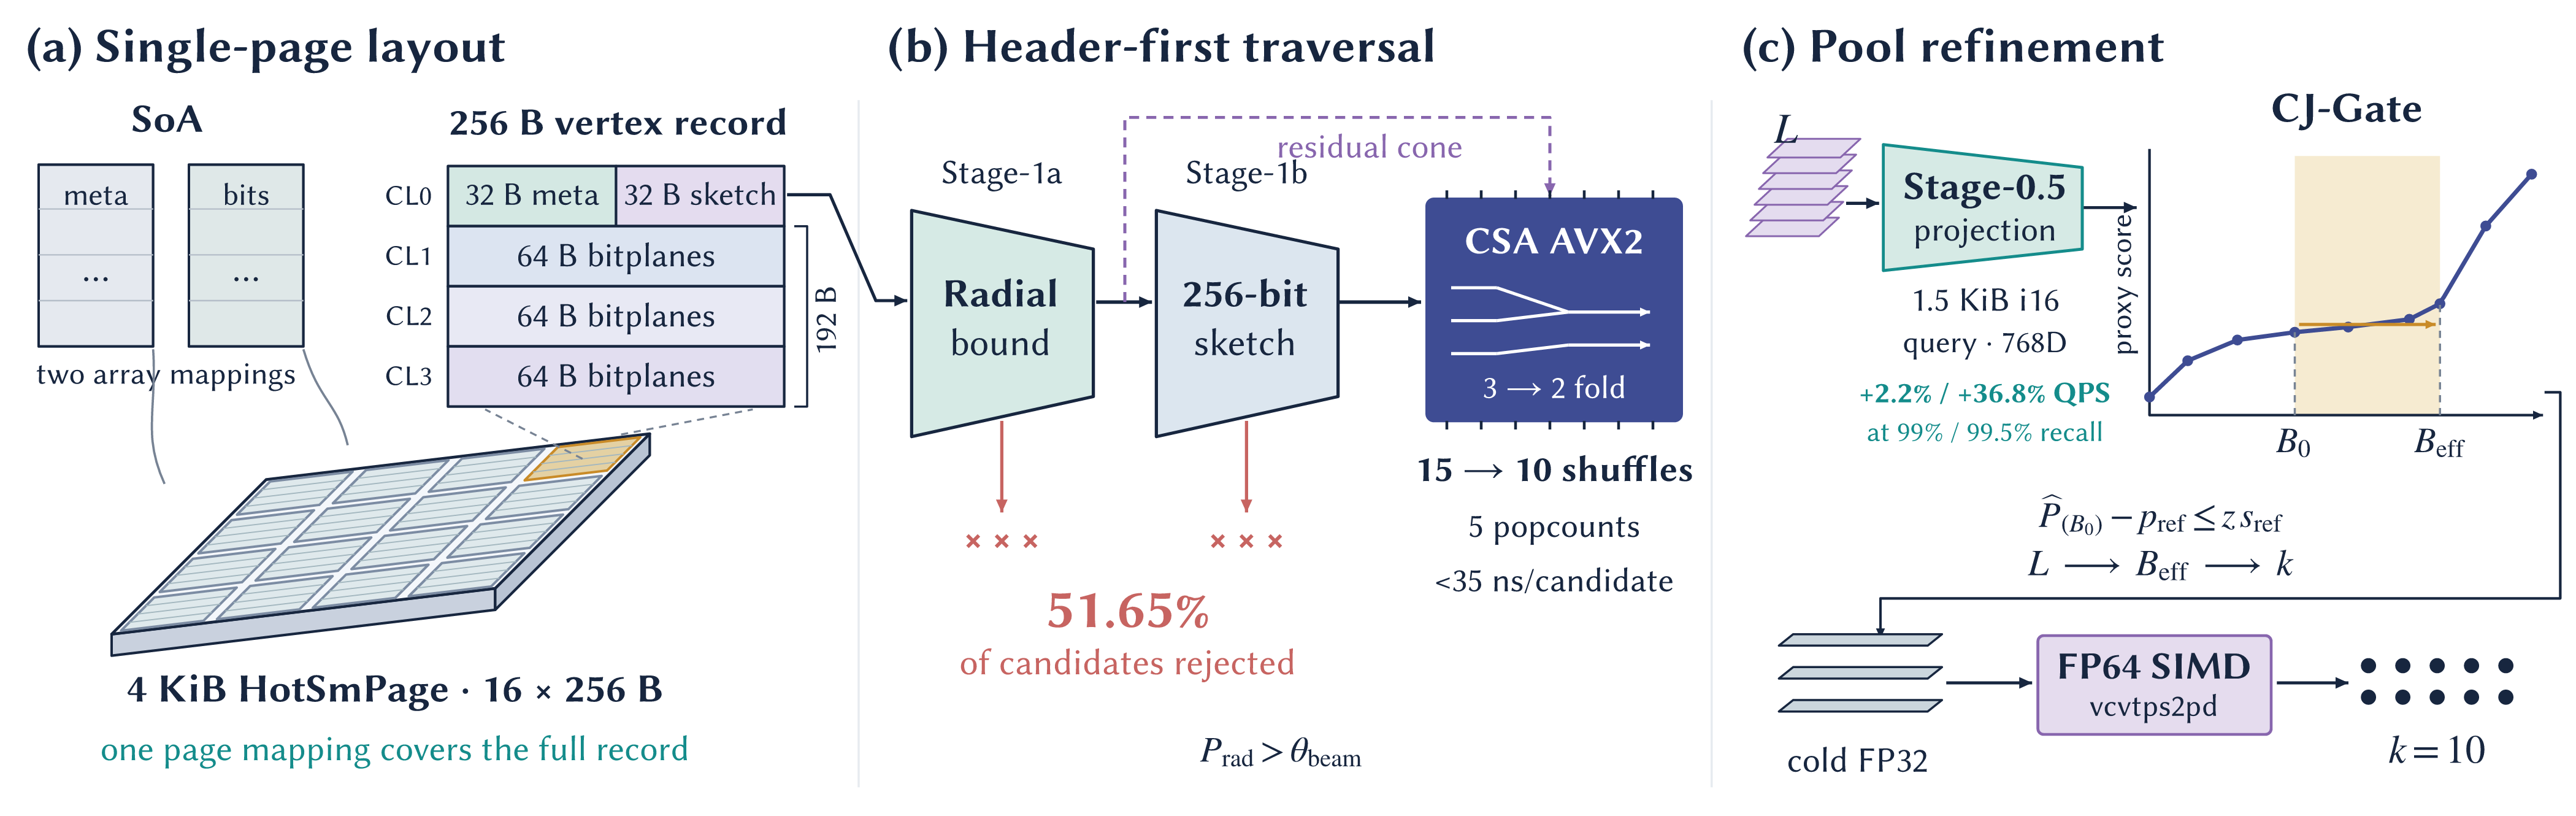
\includegraphics[width=\textwidth]{pelorus_execution.png}
  \caption{Header-first query execution at $D=768$. (a)~One $4$\,KiB page contains 16 records, each with a 64\,B header and 192\,B bitplanes. (b)~Radial and sketch gates precede full bitplane reads, with residual vertices bypassing the sketch gate. The skip rate and kernel annotations use the {Cohere-1M} measurements. (c)~Asymmetric projection precedes adaptive rerank admission and cold-vector FP64 evaluation. The score curve is schematic. \textsc{Stage-0.5} improves $99.5\%$-recall {Cohere} QPS by $58.2\%$ in the controlled ablation. The measured $+63.7\%$ ({Cohere}, $99.5\%$ recall) and $+76.5\%$ ({MERU}, $99\%$ recall) gains combine \textsc{CJ-Gate} with stabilized sketching.}
  \label{fig:execution_overview}
\end{figure*}

Figure~\ref{fig:execution_overview} follows a query from page translation to final reranking. On million-scale hyperbolic graphs, reaching $99\%$ Recall@10 at $L \in [128, 256]$ expands $300\text{--}350$ vertices and scores $4{,}500\text{--}5{,}800$ neighbors per query while reading only $B \in [64, 128]$ cold FP32 vectors in reranking.
Latency is thus governed by random {DTLB} walks, cache-line traffic, and 2-bit popcounts.
Query-private scratch buffers reset via generation stamps across requests, while scoring depends only on the query and immutable index state.

\subsection{Single-Page Co-Location and Variance-Stabilized Sketching}
\label{subsec:colocated_page}
\label{subsec:symsketch}

In Structure-of-Arrays ({SoA}) layouts, polar headers ($32$\,MB at $N=10^6$) and 2-bit bitplanes ($192$\,MB at $D=768$) live in separate arrays (whereas disk reorderers~\cite{wang2024starling} and neighbor-embedded codes~\cite{gou2025symphonyqg} renumber vertices or duplicate codes).
Because x86-64 cores hold only $64\text{--}96$ L1 and $1{,}024\text{--}3{,}072$ L2 {DTLB} entries for $4$\,KiB pages, $5{,}500$ random hops over $224$\,MB incur two page walks per candidate under {SoA}.

\begin{table}[t]
  \centering
  \caption{Page-aligned $4096$\,B \texttt{HotSmPage} with power-of-two record stride $S_{\mathrm{rec}} = \operatorname{next\_pow2}(64 + 16\lceil D/64\rceil)$\,B ($D=768$: $S_{\mathrm{rec}} = 256$\,B, $K = 16$ vertices/page). Resolving the $64$\,B \texttt{HotSmHeader} translates the entire vertex record on the same $4$\,KiB OS page.}
  \label{tab:hot_sm_page}
  \footnotesize
  \setlength{\tabcolsep}{4pt}
  \begin{tabularx}{\linewidth}{@{}l>{\raggedright\arraybackslash}Xr@{}}
    \toprule
    \textbf{Offset} & \textbf{Per-Vertex Slot in $4096$\,B \texttt{HotSmPage} ($D=768$)} & \textbf{Size} \\
    \midrule
    \texttt{0x00..0x1F} & \texttt{PolarNodeMeta} (radial, {SM}, \& cone scalars) & $32$\,B \\
    \texttt{0x20..0x3F} & \texttt{SymSketch256} ($4 \times \texttt{u64}$ strided sign sketch) & $32$\,B \\
    \texttt{0x40..0x9F} & Positive-sign {SM} bitplane (\texttt{pos}, $12 \times \texttt{u64}$) & $96$\,B \\
    \texttt{0xA0..0xFF} & Strong-magnitude {SM} bitplane (\texttt{strong}, $12 \times \texttt{u64}$) & $96$\,B \\
    \bottomrule
  \end{tabularx}
\end{table}

Table~\ref{tab:hot_sm_page} shows \texttt{HotSmPage}: each vertex occupies $S_{\mathrm{rec}} = \operatorname{next\_pow2}(64 + 16\lceil D/64\rceil)$\,B ($256$\,B at $D=512, 768$ with $K=16$ vertices/page, $512$\,B at $D=1536$ with $K=8$, and $128$\,B at $D=20$ with $K=32$, up to $D=16{,}128$).
Since $S_{\mathrm{rec}}$ divides $4096$ ($\text{page\_id} = \text{vid}/K$, $\text{slot} = \text{vid} \bmod K$), the 64-byte \texttt{HotSmHeader} (\texttt{PolarNodeMeta} + \texttt{SymSketch256}) and trailing bitplanes share one $4$\,KiB OS page and virtual-page translation for supported dimensions ($D \le 16{,}128$), avoiding cross-array secondary page-table walks per vertex access.

To avoid reading trailing bitplane cache lines ($3$ lines at $D=768$, $6$ at $D=1536$) once the $L$-th beam bound $\theta_{\mathrm{beam}}$ tightens, \rquiver{} prefetches only the $64$\,B \texttt{HotSmHeader} and applies two gates:
(1)~\textbf{Stage-1a (Radial Lower-Bound Gate)} discards $v$ if $P_{\mathrm{rad}}(r_q, r_v) = (r_q - r_v)^2 f_q f_v > \theta_{\mathrm{beam}}$ (Proposition~\ref{prop:geodesic_apex}(1)).
(2)~\textbf{Stage-1b (\texttt{SymSketch256} Gate)} uses four \texttt{u64} \texttt{XOR}+\texttt{POPCNT} instructions to get the 256-bit Hamming distance $H$, indexing $2$\,KB L1 tables for $\hat{\gamma}_{256} = \cos(\pi H / 256)$ and the binomial ratio $\rho_{\mathrm{std}}(H) = \max(1, \sigma_{\mathrm{sk}}(H/256)/\sigma_{\mathrm{sk}}(48/256))$ (Proposition~\ref{prop:asym_cj_gate}(3)) to prune non-residual vertices once the beam fills whenever $R(r_q, r_v) + W(r_q, r_v)(1 - \min(1, \hat{\gamma}_{256} + \Delta_0\rho_{\mathrm{std}}(H))) > \theta_{\mathrm{beam}}$.
On {Cohere-1M}, Stage-1a/1b skip $57.6\%$ of bitplane loads, lifting 1T $99\%$-recall QPS from $1{,}752$ ({SoA}) to $1{,}909$ (\texttt{HotSmPage}) and $2{,}071$ ($+18.2\%$).

\subsection{3-to-2 Carry-Save AVX2 Bitplane Kernel}
\label{subsec:csa_kernel}

Surviving neighbors evaluate Lemma~\ref{lem:sm_pythagorean}'s five-popcount product followed by~\eqref{eq:sm_calibration} using header scalars $(a, \delta, \sigma, s)$.
Global vertices score $(u_q, u_v)$ directly; residual vertices bypass Stage-1b after Stage-1a, cache $(\alpha_{q,c}, \beta_{q,c})$ ($\le 512$ axis projections/query), return $\alpha_{q,c}\alpha_v$ if degenerate, reuse or materialize unit $\tilde{r}_{q,c}$ ($\le 16$ slots when cached or $|\alpha_{q,c}| \ge 0.20, \beta_{q,c} > 10^{-6}$ with a free slot) for $\operatorname{clip}_{[-1,1]}(\alpha_{q,c}\alpha_v + \beta_{q,c}\beta_v t)$, and otherwise use the global-query/residual branch $\operatorname{clip}_{[-1,1]}(\alpha_{q,c}\alpha_v + \beta_v t)$ (full dispatch in the supplemental material).
With $x = s_q \oplus s_v$, the five counts $\popcnt(x)$, $\popcnt(x \wedge m_q)$, $\popcnt(x \wedge m_v)$, $\popcnt(m_q \wedge m_v)$, and $\popcnt(x \wedge m_q \wedge m_v)$ require $15$ {AVX2} \texttt{vpshufb} shuffles~\cite{mula2018faster} at $D=768$ if evaluated independently.
Adapting bitwise carry-save reduction~\cite{mula2018faster}, \rquiver{} folds triplets $(A, B, C)$ in 256-bit \texttt{YMM} registers via a \emph{3-to-2 Carry-Save Adder} ({CSA}):
\begin{equation}
  \mathrm{Sum} = A \oplus B \oplus C, \qquad
  \mathrm{Carry} = (A \wedge B) \vee \bigl((A \oplus B) \wedge C\bigr),
  \label{eq:csa_identity}
\end{equation}
where $\popcnt(A) + \popcnt(B) + \popcnt(C) = \popcnt(\mathrm{Sum}) + 2\,\popcnt(\mathrm{Carry})$, cutting \texttt{vpshufb} shuffles by $33\%$ ($15 \to 10$) to score a $768$D candidate in $<35$\,ns with distance-2 prefetching.

\subsection{Asymmetric Projection, \textsc{CJ-Gate}, and FP64 Reranking}
\label{subsec:stage05_rerank}

\begin{proposition}[Deterministic Orthogonal-Projection Estimator, Off-Axis {CJ-Gate}, and Sketch Variance]
\label{prop:asym_cj_gate}
Let $\hat{u}_v$ be the two-level {SM} code of $u_v \in \Sunit$ with $\sigma_v^2 = \|\hat{u}_v\|_2^2 = \langle u_v, \hat{u}_v\rangle$ (Lemma~\ref{lem:sm_pythagorean}). Then:
(1)~\textbf{Deterministic orthogonal projection:} Writing $u_q = \gamma_{qv} u_v + w$ ($\langle w, u_v\rangle = 0$), every pair $u_q, u_v \in \Sunit$ satisfies without rotational or distributional assumptions:
\begin{equation}
  \langle u_q, \hat{u}_v\rangle / \sigma_v^2 = \gamma_{qv} + \langle w, \hat{u}_v - \sigma_v^2 u_v\rangle / \sigma_v^2,
  \label{eq:orth_proj_asym}
\end{equation}
recovering $\gamma_{qv}$ with zero shrinkage along $u_v$ (whereas {RaBitQ}'s $\langle \bar{o}, o\rangle$ divisor~\cite{gao2024rabitq} achieves unbiasedness in expectation via global random rotations).
(2)~\textbf{Off-axis Conformal Jacobian (\textsc{CJ-Gate}):} Propagating $\sigma_\gamma(q, v) = \sqrt{\kappa_{\mathrm{SM}}/D}\,\tilde{\beta}(q, v)$ ($\tilde{\beta} = \beta_{q,c}\beta_v$ under~\eqref{eq:cone_estimator}, $\tilde{\beta} = \beta_v$ on unmaterialized cones, and $\tilde{\beta} = 1$ globally) through~\eqref{eq:polar_proxy} gives
\begin{equation}
  \sigma_P(q, v) = \bigl|\partial P_{\mathbb{B}} / \partial \gamma_{qv}\bigr|\sigma_\gamma(q, v) = 2 r_q r_v f_q f_v \sqrt{\kappa_{\mathrm{SM}}/D}\,\tilde{\beta}(q, v),
  \label{eq:cj_sigma}
\end{equation}
whereas $\beta_v^2$ in place of $\beta_{q,c}\beta_v$ underestimates $\sigma_P$ by up to $5.49\times$ ($\alpha_v = 0.995, \alpha_{q,c} = 0.84$).
(3)~\textbf{Sketch variance ratio:} Under $H \sim \operatorname{Binomial}(B_s, p)$ ($B_s = 256$, $\hat{\gamma}_{B_s} = \cos(\pi p)$), delta propagation gives $\sigma_{\mathrm{sk}}(p) = \frac{\pi}{\sqrt{B_s}}\sin(\pi p)\sqrt{p(1 - p)}$, inflating by $2.265\times$ at $H = 115$ ($2.306\times$ max at $H = 128$) relative to $H_{\mathrm{ref}} = 48$.
\end{proposition}
\begin{proof}[Proof Sketch]
Applying $\langle u_v, \hat{u}_v\rangle = \sigma_v^2$ and $\langle w, u_v\rangle = 0$ to $\langle \gamma_{qv} u_v + w, \hat{u}_v\rangle$ proves~\eqref{eq:orth_proj_asym}. Next, $|\partial P_{\mathbb{B}}/\partial \gamma_{qv}| = W(r_q, r_v)$ gives~\eqref{eq:cj_sigma}, and $|\frac{\mathrm{d}}{\mathrm{d}p}\cos(\pi p)|\sqrt{p(1-p)/B_s}$ gives $\sigma_{\mathrm{sk}}(p)$ (full derivations in the supplemental material).
\end{proof}

Once beam search converges to pool $\mathcal{P}$ ($|\mathcal{P}| = L$), \rquiver{} avoids reading all $L$ cold FP32 vectors via three steps:
(1)~\textbf{L1-Bounded \textsc{Stage-0.5} Re-Scoring:} Evaluating $\hat{\gamma}_{\mathrm{asym}}(u_q, u_v) = \operatorname{clip}_{[-1,1]}(\langle u_q, \hat{u}_v\rangle / \sigma_v^2)$ with unquantized $u_q$ ($e_q = 0$) removes cross-shell query variance (Theorem~\ref{thm:conformal_flip}(2)) and shrinkage (Proposition~\ref{prop:asym_cj_gate}(1)), using $\langle u_q, \hat{u}_v\rangle = a_v(2 S_+ - S_{\mathrm{tot}}) + \delta_v(2 S_{+h} - S_h)$ over $S_{\mathrm{tot}} = \sum_i u_{q,i}$, $S_+ = \sum_{s_{v,i}=1} u_{q,i}$, $S_h = \sum_{m_{v,i}=1} u_{q,i}$, and $S_{+h} = \sum_{s_{v,i}=1 \land m_{v,i}=1} u_{q,i}$.
Unlike 4-bit nibble {SIMD} tables~\cite{andre2015cache,andre2017accelerated,trent2024bbq}, \texttt{AsymQuerySm} quantizes $u_q$ once into a $1.5$\,KiB L1-resident \texttt{i16} array ($q_{\mathrm{i16},i} = \operatorname{round}(8100\,u_{q,i})$ at $D=768$, keeping 16-lane sums $\le 32{,}408 < 2^{15}-1$) and accumulates $(S_+, S_h, S_{+h})$ via {AVX2} bit-mask selection and \texttt{vpmaddwd} (lazily caching \texttt{AsymQuerySm}$(\tilde{r}_{q,c})$ on materialized cones).
(2)~\textbf{\textsc{CJ-Gate} Promotion:} Sorting $\mathcal{P}$ by asymmetric proxy sets $B_0 = \min(B, L)$, $j_{\mathrm{ref}} = \min(k, B_0)$, $p_{\mathrm{ref}} = \widehat{P}_{(j_{\mathrm{ref}})}$, and scale $s_{\mathrm{ref}}$ from~\eqref{eq:cj_sigma} ($\kappa_{\mathrm{SM}} = 0.221$, relative-gap $0.22 \Rightarrow z = 2$, $B_{\max} = 768$, or $\max(p_{\mathrm{ref}}, 10^{-9})\cdot 0.22$ without router metadata). If $B_0 < L$ and $\widehat{P}_{(B_0)} - p_{\mathrm{ref}} \le z\,s_{\mathrm{ref}}$, reranking extends while $\widehat{P}_{(j)} \le p_{\mathrm{ref}} + (z + 0.8)s_{\mathrm{ref}}$ and $j \le \min(L, \max(B_0, B_{\max}))$.
(3)~\textbf{FP64 {SIMD} Reranking:} Cold vectors $v_{(j)}$ widen via \texttt{vcvtps2pd} into {AVX-512F}/{AVX2+FMA} FP64 accumulators to evaluate exact $P_{\mathbb{B}}(q, v_{(j)})$ near $\|v\|_2 \to 1/\sqrt{c}$, invoking $\asinh$~\eqref{eq:proxy_to_geodesic} only on the final $k = 10$ results.

% 第五章：实验评估（精修投稿版——完整保留真实与合成主证据、消融与 Uniform-Narrow 适用边界，消除重复表格）
\section{Experimental Evaluation}
\label{sec:eval}

\subsection{Experimental Setup}
\label{subsec:eval_setup}

\paragraph{Hardware and Protocol.}
Experiments run in isolated Linux containers with {AMD EPYC 9654} ({Zen~4}) CPUs, each restricted via cgroups to 32 logical CPUs and $60$\,GiB RAM (swap off, {THP} \texttt{never} with $4$\,KiB pages, one job per container, native {AVX-512F}/{AVX2+FMA} Rust builds, $M = 16, M_0 = 32, L_c = 128, \alpha = 1.2$, $32$ build threads). In the main comparisons, the cold FP32 rerank store ($3{,}072$\,MB at $N=1\text{M}, D=768$) resides in RAM alongside the hot navigation index.
Following standard ANN evaluation practice~\cite{aumuller2020annbenchmarks,simhadri2022results}, we report throughput tables and curves from the first build per configuration (seed \texttt{12345} where supported, upstream randomization for HDB). Each thread count uses the fastest measured point meeting its recall target. A repeatability check over $210$ operating points and three seeds found at most $0.22$\,pp variation in recall and $\pm2.64\%$ in Core QPS at $99\%$ recall on Cohere ($\pm0.20\%$ on MERU).

\paragraph{Fixed Parameters and Operating-Point Selection.}
Full-method sweeps scan $L\in\{32,\allowbreak64,\allowbreak96,\allowbreak128,\allowbreak192,\allowbreak200,\allowbreak208,\allowbreak256,\allowbreak384,\allowbreak512,\allowbreak768,\allowbreak1024,\allowbreak1536,\allowbreak2048\}$, $B \in \{32, 64, 128\}$ ($B \le L$), and $\Delta_0 \in \{0.08, 0.12, 0.20\}$ (controls add full-pool reranking and sketch-off paths), with fixed build/purity/\textsc{CJ-Gate} constants across datasets (settings in supplemental material).
{MERU-1M}, {OpenAI-1536}, {WordNet-Hazy}, and the synthetic datasets use disjoint $2{,}000$-query tuning sets. For {Cohere-1M}, we use the $1{,}000$ public {VectorDBBench} queries and compute exact top-10 neighbors over the mapped database in FP64. For each method and thread count, the {Cohere-1M} frontier reports the highest measured QPS meeting each recall threshold on these queries.

\begin{table}[t]
  \centering
  \caption{Hyperbolic benchmarks in $\Bunit$ ($c=1$), ordered from native to mapped real workloads and clustered to isotropic synthetic stress sets.}
  \label{tab:datasets}
  \footnotesize
  \setlength{\tabcolsep}{3pt}
  \begin{tabularx}{\linewidth}{@{}lrrr>{\raggedright\arraybackslash}X@{}}
    \toprule
    \textbf{Dataset} & $N$ & $D$ & $|Q|$ & \textbf{Manifold Geometry} \\
    \midrule
    MERU-1M~\cite{astrmira2026meruimagenet1m} & 1,000K & 512 & 10,000 & Native {Lorentz}$\to\Bunit$ multimodal \\
    WordNet-Hazy & 83.9K & 20 & 2,000 & Native {Lorentz}$\to\mathbb{B}_1^{20}$ taxonomy \\
    Cohere-1M & 1,000K & 768 & 1,000 & Mapped Wikipedia ($\exp_0^1$, $\rho_{0.01}=1.44$) \\
    OpenAI-1536 & 990K & 1,536 & 8,000 & Mapped DBpedia ($\exp_0^1$, $\text{med}\,\rho=2.0$) \\
    \midrule
    Clustered-Narrow & 1,000K & 512 & 2,000 & $256$ tight cones, $\rho \in [3.9, 4.1]$ \\
    Clustered-Wide & 1,000K & 512 & 2,000 & $256$ tight cones, $\rho \in [0.4, 6.0]$ \\
    Uniform-Narrow & 1,000K & 512 & 2,000 & Isotropic $\mathbb{S}^{511}$, $\rho \in [3.9, 4.1]$ \\
    Uniform-Wide & 1,000K & 512 & 2,000 & Isotropic $\mathbb{S}^{511}$, $\rho \in [0.4, 6.0]$ \\
    \bottomrule
  \end{tabularx}
\end{table}

\paragraph{Benchmarks and Baselines.}
Table~\ref{tab:datasets} lists the eight primary $\Bunit$ ($c=1$) workloads, leading with native hyperbolic embeddings.
To evaluate native hyperbolic search at million-vector scale, we constructed and released \textbf{MERU-1M}~\cite{astrmira2026meruimagenet1m} by encoding {ImageNet} images with the frozen {MERU ViT-small} encoder~\cite{desai2023meru}.
The benchmark provides one million 512-dimensional database vectors in Poincar\'e coordinates~\eqref{eq:lorentz_isometry}, disjoint sets of $2{,}000$ tuning and $10{,}000$ test queries, and exhaustive FP64 geodesic ground truth.
\textbf{WordNet-Hazy} maps $83{,}943$ $20$D {Lorentz} {WordNet} embeddings into $\mathbb{B}_1^{20}$ ($\le 2.53\times 10^{-15}$ max numerical error).
\textbf{Cohere-1M} and \textbf{OpenAI-1536} serve as derivative radial-$\tanh$ stress tests mapped from database mean $\bar{x}$ via $\Phi(x) = \tanh\bigl(\frac{s}{2}\|x - \bar{x}\|_2\bigr)\frac{x - \bar{x}}{\|x - \bar{x}\|_2}$ ($s = 2/\operatorname{median}_i(\|x_i - \bar{x}\|_2)$, clamped at $1 - 10^{-6}$ for $\rho_{0.50} = 2.0$).
On \textbf{Cohere-1M} ($s = 0.2644$, zero clipped points), norm concentration creates a hollow shell with base depths $[0.98, 3.39]$ ($\rho_{0.01}=1.45, \rho_{0.99}=2.69$) and query depths $[1.25, 2.98]$ ($\rho_{0.01}=1.44$).
\textbf{OpenAI-1536} unit-normalizes \texttt{text-embedding-3-large} {DBpedia} vectors before centering and $\Phi(x)$ ($s = 2.093$, $8{,}000$ test + $2{,}000$ tuning queries).
Each synthetic set has one million 512D vectors. Crossing angular concentration (256 tight cones or isotropic directions) with radial support ($[3.9,4.1]$ or $[0.4,6.0]$) lets us vary either factor independently.

Internally, \textbf{Polar-FP32/SQ8} use unquantized FP32 or 8-bit directions in build and search, \textbf{SameGraph-FP32/SQ8} freeze the 2-bit graph and swap only search directions, and 2-bit progression spans \textbf{\rquiver{}-Split} (no chord swaps, \texttt{HotSmPage}, or \texttt{SymSketch256}) $\to$ \textbf{\rquiver{}-Core} (adding all three under global {SM}) $\to$ \textbf{\rquiver{}} (enabling \texttt{ResidualConeDict} and \textsc{CJ-Gate}, whereas \textbf{Global-SM} disables cone rescue, \textsc{CJ-Gate}, and stabilized sketch margins).
We report \textbf{Exact-RobustPrune}~\cite{subramanya2019diskann,prokhorenkova2022hyperbolic} on {Cohere-1M} to test exact geodesic pruning on a hollow shell ($M/L_c=16/128$, $L\le2{,}048$). We test \textbf{HyperspaceDB}~\cite{glukhota2026hyperspacedb} (HDB, commit \texttt{89d0406}, Nov.\ 9, 2026, native AVX-512F Poincar\'e HNSW, FP32/FP64 dynamic/flat), \textbf{Faiss}~\cite{douze2024faiss} (\texttt{faiss-cpu 1.16.0}, \texttt{IndexHNSWFlat}), and \textbf{Milvus}~\cite{wang2021milvus} (Standalone 3.0.5, centered-IP HNSW) at $M/L_c=16/128$ and $32/256$ with 18 $ef$ values up to $4{,}096$. In this sweep HDB and Milvus return native top-10. Faiss uses FP64 rerank budgets $B\in\{0,32,128\}$ for centered IP and raw Lorentz-IP, and $B\in\{32,128\}$ for direction search. For Lorentz coordinates $(t,\mathbf{s})$, centered IP stores $(t_v-\bar t,\mathbf{s}_v)$ and queries with $(-t_q,\mathbf{s}_q)$, where $\bar t$ is the database mean time coordinate. Their dot product preserves Lorentz ordering up to the query-only offset $t_q\bar t$ before rounding. HNSW builds links using ordinary inner products between stored vectors.

\subsection{Index Construction and Polar Representations}
\label{subsec:eval_repr}

\begin{table*}[t]
  \centering
  \caption{Real-data throughput and Cohere-1M representation controls. Each configuration uses one build and 32 construction threads.}
  \label{tab:zen4_repr}
  \footnotesize
  \setlength{\tabcolsep}{3.5pt}
  \begin{tabular*}{\linewidth}{@{\extracolsep{\fill}}llrrrrrrrrrrrr@{}}
    \toprule
    & & \textbf{Build} & \textbf{Hot Nav} & \textbf{Zero-In} & \multicolumn{3}{c}{\textbf{Recall@10 $\ge 98\%$}} & \multicolumn{3}{c}{\textbf{Recall@10 $\ge 99\%$}} & \multicolumn{3}{c}{\textbf{Recall@10 $\ge 99.5\%$}} \\
    \cmidrule(lr){6-8}\cmidrule(lr){9-11}\cmidrule(lr){12-14}
    \textbf{Dataset} & \textbf{Method} & \textbf{32T\,(s)} & \textbf{(MB)} & \textbf{Islands} & \textbf{1T QPS} & \textbf{p99} & \textbf{24T QPS} & \textbf{1T QPS} & \textbf{p99} & \textbf{24T QPS} & \textbf{1T QPS} & \textbf{p99} & \textbf{24T QPS} \\
    \midrule
    \multicolumn{14}{@{}l}{\textbf{(a) Real-world workloads: native hyperbolic (MERU-1M, WordNet-Hazy) and mapped hyperbolic (Cohere-1M, OpenAI-1536)}} \\
    MERU-1M & \textbf{\rquiver{}} & 25.7 & 516.8$^*$ & 0 & 2,547 & 0.50 & 53,483 & 2,547 & 0.50 & 53,483 & 1,669 & 0.81 & 36,092 \\
    WordNet-Hazy & \textbf{\rquiver{}} & 1.5 & 32.8$^*$ & 0 & 4,130 & 0.29 & 89,847 & 3,089 & 0.38 & 65,405 & 2,341 & 0.49 & 52,371 \\
    Cohere-1M & \textbf{\rquiver{}} & 35.0 & 517.0$^*$ & 0 & 2,907 & 0.41 & 58,162 & 1,930 & 0.62 & 42,466 & 738 & 1.65 & 17,137 \\
    OpenAI-1536 & \textbf{\rquiver{}} & 43.6 & 765.6$^*$ & 0 & 1,378 & 1.03 & 25,725 & 792 & 1.81 & 14,731 & 481 & 3.05 & 9,094 \\
    \midrule
    \multicolumn{14}{@{}l}{\textbf{(b) Controlled internal representation comparison on Cohere-1M (end-to-end 1T + 24T)}} \\
    \multirow{5}{*}{Cohere-1M}
     & Polar-FP32 & 197.7 & 3,373.0$^\ddagger$ & 0 & 1,048 & 1.17 & 15,063 & 457 & 2.63 & 7,004 & 265 & 4.33 & 3,928 \\
     & Polar-SQ8 & 68.3 & 1,069.0$^\ddagger$ & 0 & 1,818 & 0.75 & 36,304 & 858 & 1.56 & 16,488 & 396 & 3.25 & 7,353 \\
     & \rquiver{}-Split & \textbf{32.2} & \textbf{485.0} & 628 & 2,765 & 0.43 & 56,828 & 1,739 & 0.72 & 37,747 & 617 & 1.84 & 14,393 \\
     & \rquiver{}-Core & 32.8 & 517.0$^*$ & 0 & \textbf{3,800} & \textbf{0.31} & \textbf{73,861} & \textbf{2,003} & \textbf{0.59} & \textbf{46,796} & 687 & \textbf{1.64} & 16,029 \\
     & \textbf{\rquiver{}} & 35.0 & 517.0$^*$ & \textbf{0} & 2,907 & 0.41 & 58,162 & 1,930 & 0.62 & 42,466 & \textbf{738} & 1.65 & \textbf{17,137} \\
    \bottomrule
  \end{tabular*}
  \par\vspace{1pt}
  {\scriptsize \textit{Note:} Hot Nav measures active traversal memory (excluding the shared $3{,}072.0$\,MB cold FP32 rerank store for 2-bit/SQ8); 1T p99 in ms. $^*$Includes \texttt{HotSmPage} and sketch. The corresponding split layouts without sketches use $420.8$, $26.1$, $485.0$, and $670.6$\,MB on MERU, WordNet-Hazy, Cohere, and OpenAI, respectively. $^\ddagger$Active SQ8/FP32 totals ($+8.0$\,MB inv.\ norms; raw benchmark counters kept unaccessed $192.0$\,MB 2-bit bitplanes, reading $1{,}261.0$/$3{,}565.0$\,MB; Table~\ref{tab:node_layout}). The $98\%$ and $99\%$ MERU entries select the same configuration.}
\end{table*}

On {MERU-1M}, $(L,B,\Delta_0)=(128,128,0.20)$ gives $99.252\%$ recall at $2{,}547$/$53{,}483$\,QPS (1T/24T). At $L=256$, recall is $99.758\%$ at $1{,}669$/$36{,}092$\,QPS. All four real-data graphs have zero islands and zero active cones (Table~\ref{tab:zen4_repr}a).

On {Cohere-1M}, construction takes $35.0$\,s for \rquiver{} and $197.7$\,s for Polar-FP32. Hot navigation occupies $517$ versus $3{,}373$\,MB ($3{,}589$\,MB including cold vectors for \rquiver{}). At $98\%$, Core selects $(64,64,0.20)$ and full \rquiver{} selects $(96,64,0.12)$. At the latter setting Core serves $3{,}230$\,QPS at $98.24\%$ and the full method $2{,}907$ at $98.27\%$. Core also leads at the $99\%$ target. The full method leads at $99.5\%$ on both thread counts.

\subsection{Comparison with Hyperbolic and Flat-Proxy Engines}
\label{subsec:eval_external}

\begin{table*}[t]
  \centering
  \caption{Measured comparison of \rquiver{} and external baselines on native {MERU-1M} and mapped {Cohere-1M} (Zen~4, 32 build threads; 1T and 24T).}
  \label{tab:external_baselines}
  \scriptsize
  \setlength{\tabcolsep}{1.5pt}
  % 原生双曲（MERU-1M 优先）与高维空心映射（Cohere-1M）外部对照分区精排总表（消除无关全空占位列）
\begin{tabular*}{\linewidth}{@{\extracolsep{\fill}}llrrrrrrrrrrrrr@{}}
\multicolumn{15}{@{}l}{\textbf{(a) MERU-1M (Native Hyperbolic, $512$D, $10{,}000$ queries; main-sweep methods reaching $99.5\%$ Recall@10)}} \\
\toprule
 & & \textbf{Build} & \textbf{Peak} & \multicolumn{5}{c}{\textbf{1-Thread QPS at Recall@10}} & \textbf{1T p99} & \multicolumn{5}{c}{\textbf{24-Thread QPS at Recall@10}} \\
\cmidrule(lr){5-9}\cmidrule(lr){11-15}
\textbf{Method} & \textbf{$M/L_c$} & \textbf{32T\,(s)} & \textbf{Rec@10} & \textbf{$\ge90\%$} & \textbf{$\ge95\%$} & \textbf{$\ge98\%$} & \textbf{$\ge99\%$} & \textbf{$\ge99.5\%$} & \textbf{(ms)} & \textbf{$\ge90\%$} & \textbf{$\ge95\%$} & \textbf{$\ge98\%$} & \textbf{$\ge99\%$} & \textbf{$\ge99.5\%$} \\
\midrule
\textbf{\rquiver{}} & 16/128 & \textbf{25.7} & 99.983\% & \textbf{5,846} & \textbf{4,521} & \textbf{2,547} & \textbf{2,547} & \textbf{1,669} & \textbf{0.50} & \textbf{94,846} & \textbf{94,846} & \textbf{53,483} & \textbf{53,483} & \textbf{36,092} \\
HDB FP32 flat & 16/128 & 87.6 & 99.947\% & 3,187 & 2,184 & 1,579 & 1,296 & 966 & 1.15 & 26,235 & 26,235 & 19,434 & 15,890 & 11,699 \\
HDB FP32 dynamic & 16/128 & 86.5 & 99.947\% & 3,136 & 2,103 & 1,493 & 1,188 & 875 & 1.27 & 30,015 & 30,015 & 18,413 & 13,780 & 11,038 \\
HDB FP64 dynamic & 32/256 & 631.4 & 99.955\% & 615 & 428 & 281 & 196 & 165 & 8.83 & 9,588 & 9,588 & 6,121 & 4,098 & 3,414 \\
HDB FP64 flat & 32/256 & 633.9 & 99.707\% & 480 & 320 & 186 & 93 & 46 & 21.68 & 6,362 & 6,362 & 4,039 & 1,933 & 925 \\
Faiss direction & 16/128 & 48.8 & \textbf{100.000\%} & 3,460 & 1,814 & 1,480 & 1,078 & 1,078 & 1.30 & 43,798 & 43,798 & 19,883 & 14,967 & 9,866 \\
Faiss centered IP & 32/256 & 99.2 & 99.988\% & 4,312 & 2,800 & 1,903 & 1,059 & 872 & 1.43 & 33,189 & 33,189 & 22,488 & 13,005 & 9,349 \\
Milvus centered IP & 32/256 & 271.6 & 99.991\% & 297 & 297 & 297 & 260 & 233 & 5.30 & 1,208 & 1,208 & 1,208 & 1,130 & 1,088 \\
\bottomrule
\end{tabular*}
\par\smallskip
\begin{tabular*}{\linewidth}{@{\extracolsep{\fill}}lrrrrrr@{}}
\multicolumn{7}{@{}l}{\textbf{MERU-1M log-map and quantized controls ($99\%$ validation target, 10,000 test queries)}}\\
\toprule
& \multicolumn{3}{c}{1 thread} & \multicolumn{3}{c}{24 threads}\\
\cmidrule(lr){2-4}\cmidrule(l){5-7}
Method & Recall@10 (\%) & QPS & p99 (ms) & Recall@10 (\%) & QPS & p99 (ms)\\
\midrule
Faiss FP32 (log-map $L_2$) & 99.059 & 2,136 & 0.65 & 99.150 & 15,103 & 2.61\\
Faiss SQ8 (log-map $L_2$) & 99.119 & 1,220 & 1.07 & 99.119 & 26,786 & 1.28\\
Milvus SQ8 (centered IP) & 99.405 & 73 & 20.75 & 99.716 & 587 & 115.23\\
HDB SQ8 (Poincar\'e, FP64 rerank) & 99.224 & 763 & 1.85 & 99.224 & 13,620 & 2.52\\
Tangent 2-bit (paired engine) & 99.107 & 1,510 & 0.99 & 99.107 & 35,813 & 0.99\\
\rquiver{} 2-bit (paired engine) & 99.248 & 2,311 & 0.55 & 99.247 & 50,848 & 0.60\\
\bottomrule
\end{tabular*}

\par\vspace{3pt}
\begin{tabular*}{\linewidth}{@{\extracolsep{\fill}}llrrrrrrrrrr@{}}
\multicolumn{12}{@{}l}{\textbf{(b) Cohere-1M (Mapped Hollow Shell, $768$D, $1{,}000$ queries; baselines reaching $\ge95\%$ Recall@10)}} \\
\toprule
 & & \textbf{Build} & \textbf{Peak} & \multicolumn{4}{c}{\textbf{1-Thread QPS at Recall@10}} & \multicolumn{4}{c}{\textbf{24-Thread QPS at Recall@10}} \\
\cmidrule(lr){5-8}\cmidrule(lr){9-12}
\textbf{Method} & \textbf{$M/L_c$} & \textbf{32T\,(s)} & \textbf{Rec@10} & \textbf{$\ge90\%$} & \textbf{$\ge95\%$} & \textbf{$\ge98\%$} & \textbf{$\ge99\%$} & \textbf{$\ge90\%$} & \textbf{$\ge95\%$} & \textbf{$\ge98\%$} & \textbf{$\ge99\%$} \\
\midrule
\textbf{\rquiver{}} & 16/128 & \textbf{35.0} & \textbf{99.700\%} & \textbf{4,939} & \textbf{4,939} & \textbf{2,907} & \textbf{1,930} & \textbf{96,584} & \textbf{96,584} & \textbf{58,162} & \textbf{42,466} \\
Faiss centered IP & 32/256 & 167.3 & 98.910\% & 1,652 & 830 & 127 & \missing & 10,717 & 10,717 & 1,660 & \missing \\
Milvus centered IP & 32/256 & 361.7 & 98.690\% & 252 & 238 & 76 & \missing & 1,115 & 1,115 & 999 & \missing \\
HDB FP32 dynamic & 32/256 & 414.8 & 96.780\% & 839 & 290 & \missing & \missing & 3,416 & 3,416 & \missing & \missing \\
HDB FP32 flat & 32/256 & 416.3 & 96.670\% & 946 & 279 & \missing & \missing & 3,656 & 3,656 & \missing & \missing \\
\bottomrule
\end{tabular*}

  \par\vspace{1pt}
  {\scriptsize HDB = HyperspaceDB. Dashes mark unmet targets ($ef\le4{,}096$). Build and $M/L_c$ refer to the $99\%$ point or the highest recall reached. The 1T p99 is from the selected $99\%$ point. The paired-engine rows use a separate, sequentially timed comparison with validation-selected budgets. For \rquiver{}, $(L,B)$ is $(128,128)$ at 1T and $(128,32)$ at 24T. On Cohere, Exact-RobustPrune peaks at $93.94\%$, HDB FP64 at $94.43\%$, and Faiss direction/raw-IP at $65.17/0.12\%$.}
\end{table*}

\begin{figure*}[t]
  \centering
  \begin{subfigure}[t]{0.328\textwidth}
    \centering
    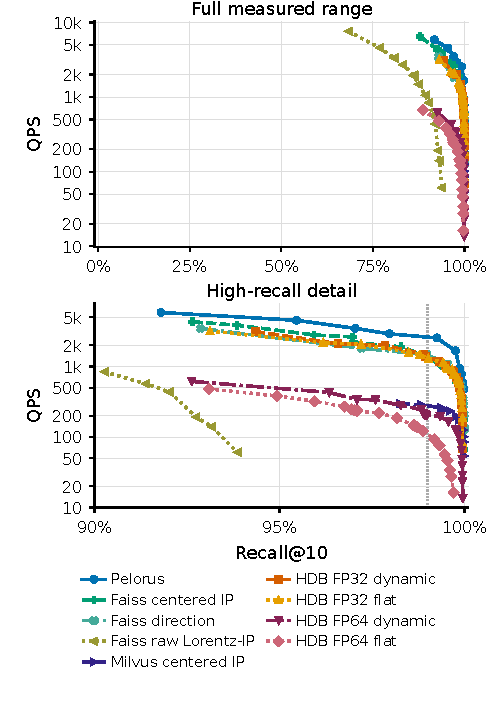
\includegraphics[width=\linewidth]{pareto_meru_1m_1t.pdf}
    \caption{MERU-1M ($512$D, 1 thread)}
    \label{fig:pareto_meru}
  \end{subfigure}\hfill
  \begin{subfigure}[t]{0.328\textwidth}
    \centering
    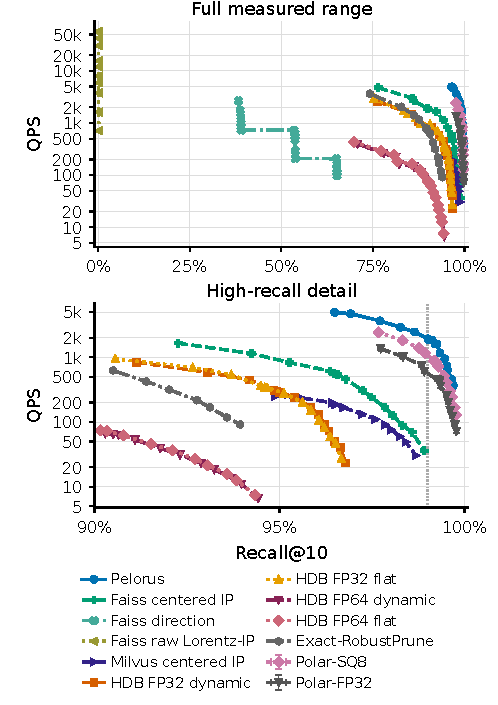
\includegraphics[width=\linewidth]{pareto_cohere_1m_1t.pdf}
    \caption{Cohere-1M ($768$D, 1 thread)}
    \label{fig:pareto_cohere}
  \end{subfigure}\hfill
  \begin{subfigure}[t]{0.30\textwidth}
    \centering
    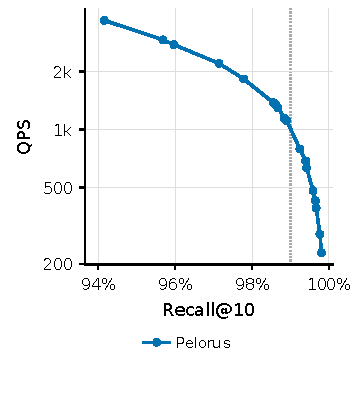
\includegraphics[width=\linewidth]{pareto_openai_1536_1t.pdf}
    \caption{OpenAI-1536 ($1536$D, 1 thread)}
    \label{fig:pareto_openai}
  \end{subfigure}
  \caption{Single-build, single-thread Recall@10--QPS frontiers on Zen~4. Panels (a,b) include external baselines. Panel (c) shows \rquiver{} on mapped {OpenAI-1536}.}
  \label{fig:real_pareto}
\end{figure*}

On native {MERU-1M} at the $99\%$ target, \rquiver{} serves $1.97\times/3.37\times$ the QPS of HDB FP32 flat and $1.19\times/3.54\times$ that of Faiss FP32 log-map $L_2$ HNSW (1T/24T, Table~\ref{tab:external_baselines}). The log-map~\cite{deng2026hyem} uses $ef=128$ with direct top-10 at 1T and 128-candidate reranking at 24T.

\paragraph{Two-bit tangent-space control.}
Both graphs use the same Rayon scheduler, 2-bit {SM} directions, degree bound and FP64 reranker. The tangent graph uses log-map norms, a single entry and isotropic RobustPrune. At $L=B=128$, it serves $2{,}326$\,QPS at $97.837\%$ recall versus $2{,}248$ at $99.248\%$ for \rquiver{} (1T). To reach $99\%$, it doubles $L$ to 256. At the validation-selected budgets, \rquiver{} serves $1.53\times/1.42\times$ its QPS (1T/24T, Table~\ref{tab:external_baselines}), using $516.8$ versus $428.0$\,MB of hot state.

\paragraph{SQ8 graph indices.}
Across both build budgets and layouts ($ef\le4{,}096$), HDB SQ8 direct top-10 peaks at $63.93/51.75\%$ (Poincar\'e/Lorentz). FP64 reranking of 128 candidates raises Poincar\'e SQ8 above $99\%$ at $ef=256$ and Lorentz SQ8 to $96.66\%$. Faiss \texttt{IndexHNSWSQ} and Milvus \texttt{HNSW\_SQ} test both retrieval modes at $M/L_c=16/128$. Faiss uses in-process C++. Milvus includes Python and gRPC.

On mapped {Cohere-1M}, \rquiver{} reaches $99.70\%$ recall. Over the $32/256$ sweeps ($ef\le4{,}096$), centered-IP {Faiss} and {Milvus} peak at $98.91\%$ and $98.69\%$, and HDB FP32 dynamic and flat at $96.78\%$ and $96.67\%$. Log-map HNSW reaches $86.42\%$ on its separate 500-query test subset.

\subsection{Multi-Threaded Scaling Efficiency}
\label{subsec:eval_scaling}

\begin{figure*}[t]
  \centering
  \begin{subfigure}[t]{0.435\textwidth}
    \centering
    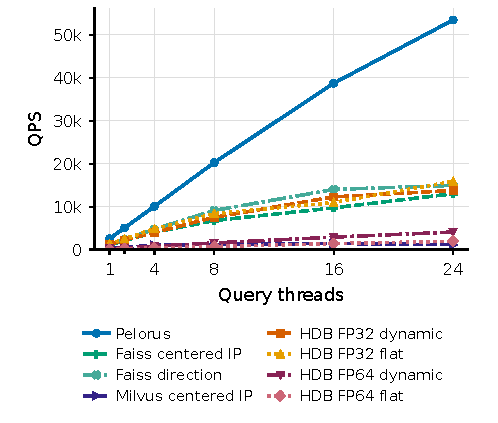
\includegraphics[width=\linewidth]{scaling_meru_1m_r99.pdf}
    \caption{MERU-1M ($\ge 99\%$ Recall)}
    \label{fig:scale_meru}
  \end{subfigure}\hfill
  \begin{subfigure}[t]{0.435\textwidth}
    \centering
    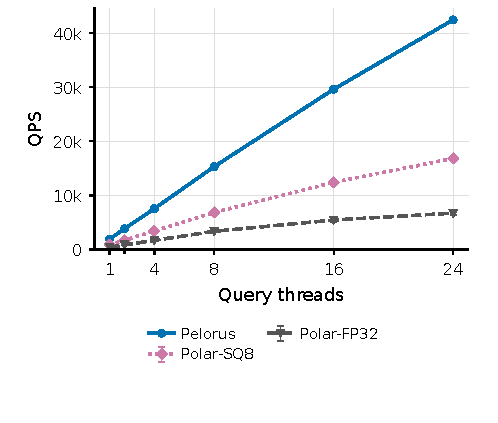
\includegraphics[width=\linewidth]{scaling_cohere_1m_r99.pdf}
    \caption{Cohere-1M ($\ge 99\%$ Recall)}
    \label{fig:scale_cohere}
  \end{subfigure}
  \caption{Single-build scaling from $1$ to $24$ query threads on Zen~4 at Recall@10 $\ge 99\%$.}
  \label{fig:scaling}
\end{figure*}

The single-build scaling curves in Figure~\ref{fig:scaling} give $21.0\times$ speedup from 1T to 24T on {MERU-1M} and $22.0\times$ on {Cohere-1M}. {WordNet-Hazy} and {OpenAI-1536} reach $21.2\times$ and $18.6\times$. On {MERU-1M}, the FP32 {HDB} and {Faiss} baselines scale by $11.6$--$12.3\times$.

\subsection{Page Layout and Cold Storage}
\label{subsec:eval_storage}

On {MERU-1M} ($D=512$), compact packing raises page occupancy from 16 to 21 vertices and cuts allocation from $244.1$ to $186.0$\,MiB. At $(L,B)=(128,64)$ both layouts return identical IDs and scores ($99.249\%$ recall). Throughput moves from $2{,}416$ to $2{,}305$\,QPS at 1T and from $47{,}470$ to $51{,}088$ at 24T. On $65{,}536$-point MERU probes, allocation falls from $16.00$ to $10.24$\,MiB at $D=384$ and from $32.00$ to $21.34$ at $D=1024$. On {Cohere-1M}, both layouts use $244.1$\,MiB. Compact/default 24T throughput is $41{,}336/53{,}323$\,QPS at $(128,64)$ and $30{,}123/32{,}965$ at $(256,128)$. Both share a page translation per record. Packing also changes cache-line placement and address calculation. Hardware miss counters were unavailable. On $20$D {WordNet-Hazy}, compact pages use $6.43$ versus $10.25$\,MiB. Sharing cold FP32 vectors for navigation instead cuts RSS from $70.5$ to $63.9$\,MiB, raises recall from $97.340$ to $99.980\%$ and lowers 1T QPS from $4{,}578$ to $4{,}076$.

\begin{table}[t]
  \centering
  \caption{Cold reranking on {MERU-1M}. The 2-bit navigation graph stays in RAM. All rows use 24 threads, a 512\,MiB SSD cache and $\Delta_0=0.20$. The last column gives SSD bytes read per timed query in KiB.}
  \label{tab:meru_ssd}
  \footnotesize
  \setlength{\tabcolsep}{3pt}
  \begin{tabular}{@{}llrrrr@{}}
    \toprule
    Cold encoding & $L/B$ & Recall@10 & QPS & p99 (ms) & KiB/q \\
    \midrule
    FP32            & 512/128 & 99.917\% & 1,886 & 48.78 & 670.85 \\
    Cartesian FP16  & 512/128 & 99.902\% & 3,282 & 17.26 & 358.32 \\
    Polar FP16      & 512/128 & 99.902\% & 3,270 & 16.83 & 361.73 \\
    \midrule
    Centered SQ8    & 64/64 & 97.519\% & 23,760 & 4.48 & 44.31 \\
    Centered SQ4    & 64/64 & 90.123\% & 33,823 & 4.09 & 21.24 \\
    \bottomrule
  \end{tabular}
\end{table}

For SSD reranking we fix one graph, tune on $2{,}000$ queries, then time each condition once on $10{,}000$ test queries after 200 warmups. Batched \texttt{io\_uring} reads have a 32\,MiB in-flight budget. Polar FP16 and centered SQ4 retain an FP64 radius. At $L=512$, both FP16 formats nearly halve SSD traffic while retaining $99.902\%$ recall (Table~\ref{tab:meru_ssd}). At $L=64$, SQ4 reads $52\%$ fewer bytes per query than SQ8 and serves $42\%$ more queries per second at a cost of $7.396$ recall points. The highest SQ4 recall among the 43 configurations retested is $91.240\%$.

At $99.917\%$ recall and 24T, offloading cold FP32 to SSD with 128\,MiB cache cuts RSS from $2.573$ to $0.825$\,GiB and QPS from $22{,}822$ to $1{,}308$. At $(164,64)$, centered SQ8 gives identical top-10 across RAM and both SSD caches ($99.003\%$ recall). RAM serves $51{,}040$\,QPS (p99 $0.62$\,ms, RSS $1.155$\,GiB). Increasing the cache from 128 to 512\,MiB cuts reads/query from $103.35$ to $10.00$, raises QPS from $2{,}749$ to $20{,}136$ and lowers p99 from $23.87$ to $7.23$\,ms. RSS rises from $0.839$ to $1.228$\,GiB.

\subsection{Geometry and Execution Ablations}
\label{subsec:eval_ablation}

\begin{figure*}[t]
  \centering
  \begin{subfigure}[t]{0.435\linewidth}
    \centering
    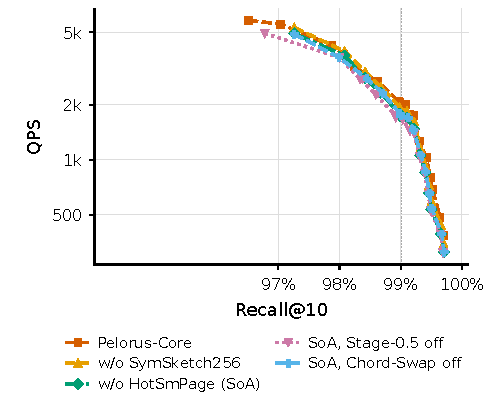
\includegraphics[width=\linewidth]{ablation_geometry_cohere_1m.pdf}
    \caption{Cohere-1M, topology and search}
    \label{fig:abl_geom}
  \end{subfigure}\hfill
  \begin{subfigure}[t]{0.435\linewidth}
    \centering
    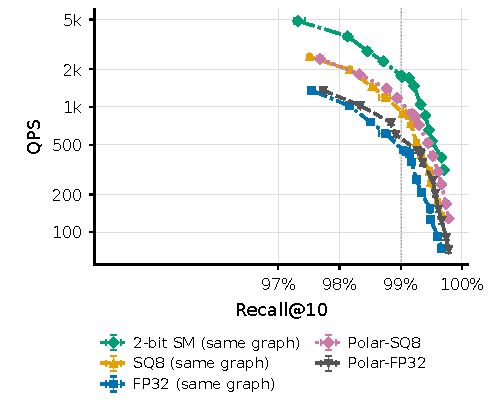
\includegraphics[width=\linewidth]{ablation_representation_cohere_1m.pdf}
    \caption{Cohere-1M, search representation}
    \label{fig:abl_repr}
  \end{subfigure}
  \par\smallskip
  \begin{subfigure}[t]{0.89\linewidth}
    \centering
    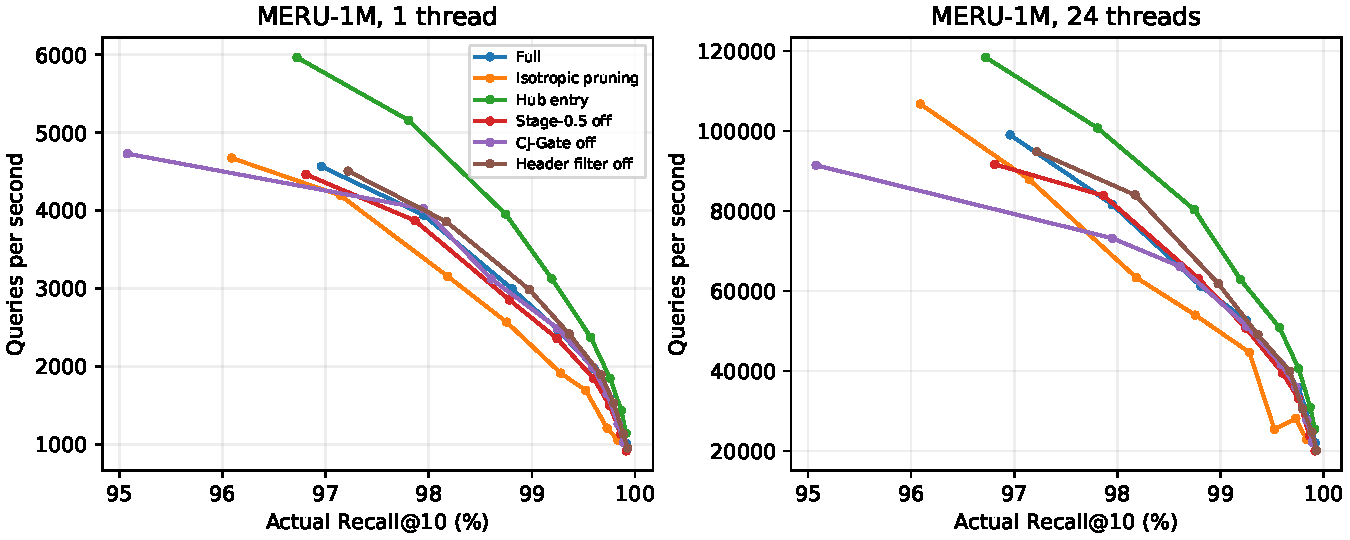
\includegraphics[width=\linewidth]{meru_ablation.pdf}
    \caption{MERU-1M, topology and search at eight fixed budgets.}
    \label{fig:abl_native}
  \end{subfigure}
  \caption{Component ablations on the first build. The upper panels give single-thread frontiers on {Cohere-1M}. The lower panels give measured recall and throughput at eight fixed budgets on {MERU-1M}.}
  \label{fig:ablation_pdf}
\end{figure*}

\paragraph{Cohere-1M}
With the Core engine and 16 budgets, QuadriPrune reaches $99\%$ at $1{,}957$\,QPS versus $426$ for the earlier two-pass policy ($L=192/1{,}536$, $B=64$). At $(192,64)$, removing the ring lowers recall from $99.00\%$ to $97.09\%$ (peak $98.74\%$). Disabling its shield gives $98.99\%$, removing the geodesic channel $99.41\%$, and removing both elevators $99.23\%$.

A simpler graph selects up to 16 of 32 links by angular diversity alone, then uses the same depth-aware refill, repair, entries and scoring. Across three paired rebuilds, QuadriPrune delivers $12$--$15\%$ more QPS at the $99\%$ target. At $99.5\%$ the angular quota delivers $35$--$66\%$ more QPS, reaching the target at $L=384$ versus $768$--$1{,}024$ ($B=128$).

At $99\%$ recall, page co-location raises single-thread throughput from $1{,}701$ to $1{,}850$\,QPS, and the sketch raises it to $2{,}003$ (Figure~\ref{fig:abl_geom}). On the split-array path, disabling \textsc{Stage-0.5} gives $1{,}665$/$391$\,QPS at $99/99.5\%$ versus $1{,}701$/$535$ with it. Chord repair connects 521 zero-in-degree vertices. In the 32-query header traces, the default sketch rejects $51.65\%$ of inspected candidates, compared with $45.82\%$ without its radial term. On one full graph, switching \textsc{CJ-Gate} preserves all returned IDs and scores at six fixed budgets. Sketch-margin calibration moves recall from $98.15$ to $97.94\%$ at $L=B=64$, and from $99.49$ to $99.52\%$ at $(768,128)$, changing which budgets meet the table thresholds.

\paragraph{MERU-1M}
Figure~\ref{fig:abl_native} uses one graph for all query switches. The isotropic control rebuilds the graph with the same degree, refill and repair. It discards candidate $v$ at $u$ if a selected $p$ satisfies $\alpha\tilde d(p,v)\le\tilde d(u,v)$, where $\tilde d$ is the geodesic distance estimate recovered from the quantized proxy. At $L=B=128$, QuadriPrune raises recall from $98.755\%$ to $99.251\%$ ($2{,}568$ to $2{,}470$\,QPS, 1T). At $(256,128)$, hub-only entry serves $1{,}848$ versus $1{,}588$\,QPS for the full router ($99.757/99.754\%$ recall). Removing \textsc{Stage-0.5} or the header filter gives $33{,}206$ or $30{,}593$\,QPS at 24T versus $35{,}872$ for the full method. Disabling \textsc{CJ-Gate} gives $36{,}031$\,QPS and $99.729\%$ recall. Jointly selecting entry and $(L,B)$ on $2{,}000$ validation queries picks hubs at all three recall targets for 1T and 24T. At the $99\%$ target they serve $2{,}868/64{,}786$\,QPS at $99.20\%$ test recall, versus $2{,}272/49{,}731$ at $99.25\%$ with fixed PolarRouter. The 16 hubs bypass both cone scans. At the $99.5\%$ validation target on Cohere, 1T selects PolarRouter at $L=512$ versus $768$ for hubs ($99.36\%$ held out).

\paragraph{Pruning channels.}
The ring matters most on hollow-shell Cohere ($-1.91$ recall points when removed), and geodesic edges on deep HyperE WordNet ($-9.02$, versus $+0.03$ on MERU). Elevators provide cross-shell links. Removing either changes WordNet recall by at most $0.25$ points, and removing both preserves the $99\%$ Cohere target. Varying ring width or elevator gap shifts recall by at most $0.43$ points. Geodesic/ring quota sweeps span $99.207$--$99.289\%$ on MERU and $67.969$--$68.945\%$ on WordNet with unchanged degree and reachability.

\subsection{Residual Coding and Recall Limits}
\label{subsec:eval_synthetic}

\begin{table*}[t]
  \centering
  \caption{Synthetic hyperbolic comparison (1M vectors, 512D, Zen~4, 32 build threads, $2{,}000$ queries): clustered high-recall~(a), wide isotropic~(b), narrow-shell limits~(c), and centered flat-proxy peak collapse~(d).}
  \label{tab:synthetic_external}
  \scriptsize
  \setlength{\tabcolsep}{1.5pt}
  % 合成极端分布按结构与召回体制拆分对照（将 120 格无效 "-" 压缩为高密度主战力区、各向同性拓宽区及边界极限对比）
\begin{tabular*}{\linewidth}{@{\extracolsep{\fill}}llrrrrrrrrrrrrrr@{}}
\multicolumn{16}{@{}l}{\textbf{(a) Clustered Boundary Cones (Clustered-Narrow \& Clustered-Wide, $90\%\text{--}99.5\%$ Recall@10)}} \\
\toprule
 & & & \textbf{Build} & \textbf{Peak} & \multicolumn{5}{c}{\textbf{1-Thread QPS at Recall@10}} & \textbf{1T p99} & \multicolumn{5}{c}{\textbf{24-Thread QPS at Recall@10}} \\
\cmidrule(lr){6-10}\cmidrule(lr){12-16}
\textbf{Dataset} & \textbf{Method} & \textbf{$M/L_c$} & \textbf{32T\,(s)} & \textbf{Rec@10} & \textbf{$\ge90\%$} & \textbf{$\ge95\%$} & \textbf{$\ge98\%$} & \textbf{$\ge99\%$} & \textbf{$\ge99.5\%$} & \textbf{(ms)} & \textbf{$\ge90\%$} & \textbf{$\ge95\%$} & \textbf{$\ge98\%$} & \textbf{$\ge99\%$} & \textbf{$\ge99.5\%$} \\
\midrule
Clustered-Narrow & \textbf{\rquiver{}}$^\ddagger$ & 16/128 & \textbf{25.3} & 99.945\% & \textbf{3,371} & \textbf{2,875} & \textbf{2,092} & \textbf{1,840} & \textbf{1,551} & \textbf{0.67} & \textbf{55,231} & \textbf{55,231} & \textbf{44,175} & \textbf{38,876} & \textbf{33,132} \\
 & HDB FP32 flat & 32/256 & 106.4 & \textbf{99.950\%} & 1,568 & 1,315 & 1,133 & 998 & 998 & 1.33 & 17,024 & 17,024 & 14,483 & 13,311 & 13,311 \\
\midrule
Clustered-Wide & \textbf{\rquiver{}}$^\ddagger$ & 16/128 & \textbf{19.4} & \textbf{99.995\%} & \textbf{4,113} & \textbf{3,572} & \textbf{3,141} & \textbf{2,704} & \textbf{2,704} & \textbf{0.44} & \textbf{72,780} & \textbf{72,780} & \textbf{70,801} & \textbf{57,144} & \textbf{57,144} \\
 & HDB FP32 flat & 32/256 & 73.7 & 99.500\% & 1,037 & 908 & 735 & 735 & 645 & 2.14 & 15,090 & 15,090 & 12,519 & 12,519 & 12,011 \\
\bottomrule
\end{tabular*}
\par\vspace{3pt}
\begin{tabular*}{\linewidth}{@{\extracolsep{\fill}}llrrrrrrrr@{}}
\multicolumn{10}{@{}l}{\textbf{(b) Isotropic Wide Shell (Uniform-Wide, thresholds $\ge90\%$ to $\ge98\%$)}} \\
\toprule
 & & \textbf{Build} & \textbf{Peak} & \multicolumn{3}{c}{\textbf{1-Thread QPS at Recall@10}} & \multicolumn{3}{c}{\textbf{24-Thread QPS at Recall@10}} \\
\cmidrule(lr){5-7}\cmidrule(lr){8-10}
\textbf{Method} & \textbf{$M/L_c$} & \textbf{32T\,(s)} & \textbf{Rec@10} & \textbf{$\ge90\%$} & \textbf{$\ge95\%$} & \textbf{$\ge98\%$} & \textbf{$\ge90\%$} & \textbf{$\ge95\%$} & \textbf{$\ge98\%$} \\
\midrule
\textbf{\rquiver{}}$^\dagger$ & 16/128 & \textbf{31.9} & \textbf{98.880\%} & \textbf{639} & \textbf{397} & \textbf{300} & \textbf{9,363} & \textbf{9,363} & \textbf{6,739} \\
HDB FP32 flat & 32/256 & 299.6 & 97.860\% & 241 & 103 & \missing & 1,727 & 1,072 & \missing \\
\bottomrule
\end{tabular*}
\par\vspace{3pt}
\begin{minipage}[t]{0.38\linewidth}
\begin{tabular*}{\linewidth}[t]{@{\extracolsep{\fill}}lrrr@{}}
\multicolumn{4}{@{}l}{\textbf{(c) Uniform-Narrow Limit}} \\
\toprule
 & \textbf{Build} & \textbf{Peak} & \textbf{$\ge90\%$ QPS} \\
\textbf{Method ($M/L_c$)} & \textbf{32T\,(s)} & \textbf{Rec@10} & \textbf{(1T / 24T)} \\
\midrule
\rquiver{}$^\dagger$ (16/128) & \textbf{46.8} & 64.735\% & \missing \\
\textbf{\rquiver{}} (32/256) & 147.5 & \textbf{95.285\%} & \textbf{65 / 1,202}$^\S$ \\
HDB flat (32/256) & 478.2 & 92.170\% & 18 / 288 \\
\bottomrule
\end{tabular*}
\end{minipage}\hfill
\begin{minipage}[t]{0.60\linewidth}
\begin{tabular*}{\linewidth}[t]{@{\extracolsep{\fill}}lrrrrrrrr@{}}
\multicolumn{9}{@{}l}{\textbf{(d) Centered Flat-Proxy Collapse Across All Four Synthetic Sets ($32/256$)}} \\
\toprule
 & \multicolumn{2}{c}{\textbf{Clust.-Nar.}} & \multicolumn{2}{c}{\textbf{Clust.-Wide}} & \multicolumn{2}{c}{\textbf{Unif.-Wide}} & \multicolumn{2}{c}{\textbf{Unif.-Nar.}} \\
\cmidrule(lr){2-3}\cmidrule(lr){4-5}\cmidrule(lr){6-7}\cmidrule(lr){8-9}
\textbf{Method} & \textbf{s} & \textbf{Peak} & \textbf{s} & \textbf{Peak} & \textbf{s} & \textbf{Peak} & \textbf{s} & \textbf{Peak} \\
\midrule
Faiss cent.\ IP & 35.2 & 21.245\% & 38.3 & 4.015\% & 140.1 & 48.640\% & 311.3 & 29.860\% \\
Milvus cent.\ IP & 146.8 & 19.525\% & 273.7 & 9.330\% & 255.1 & 54.040\% & 573.6 & 46.445\% \\
\bottomrule
\end{tabular*}
\end{minipage}

  \par\vspace{1pt}
  {\scriptsize \textit{Note:} \rquiver{} uses $M/L_c=16/128$ ($L \le 2{,}048$, exc.\ $32/256$ row in~(c)), external baselines $32/256$ ($ef \le 4{,}096$); \missing{} = $\ge 90\%$ (or $\ge 98\%$ in~(b)) unreached. $^\dagger$$0$ cones (unrescued {Global-SM} peaks at $62.41\%$, $97.93\%$). $^\ddagger$$256$ cones at $0$\,B/vertex ({Global-SM} drops to $34.22\%$, $73.87\%$). $^\S$Matched $32/256$ ($M_0=64$, $772.8$\,MB hot): at $L=3{,}072$, $92.525\%$ recall and $65.4$\,QPS (1T). At $L=4{,}096$, $95.285\%$ recall and $53.6/1{,}202$\,QPS (1T/24T).}
\end{table*}

\paragraph{External Comparisons Across Synthetic Geometries.}
At the $99\%$ target on Clustered-Narrow and Clustered-Wide, \rquiver{} serves $1.84\times$/$2.92\times$ and $3.68\times$/$4.56\times$ the 1T/24T throughput of HDB FP32 flat, respectively (Table~\ref{tab:synthetic_external}). On Uniform-Wide, \rquiver{} reaches $98.88\%$ recall, HDB $97.86\%$, and the centered flat proxies at most $54.04\%$.

\paragraph{Four-Stage Recall Audit and Tangent-Cone Gains.}
For exact top-$k$ set $G_k(q)$, visited set $V(q)$, beam pool $C_L(q) \subseteq V(q)$, rerank admissions $F_B(q) \subseteq C_L(q)$, and output $R_k(q) \subseteq F_B(q)$, recall miss decomposes telescopically with zero overlap:
\begin{equation}
  \begin{aligned}
    1-\operatorname{Recall@}k
      ={}&\underbrace{\bigl(1-\tfrac{|G_k\cap V|}{k}\bigr)}_{\mathcal L_{\mathrm{reach}}}
       +\underbrace{\tfrac{|G_k\cap(V\setminus C_L)|}{k}}_{\mathcal L_{\mathrm{beam}}}\\
       &+\underbrace{\tfrac{|G_k\cap(C_L\setminus F_B)|}{k}}_{\mathcal L_{\mathrm{gate}}}
       +\underbrace{\tfrac{|G_k\cap(F_B\setminus R_k)|}{k}}_{\mathcal L_{\mathrm{rerank}}}.
  \end{aligned}
  \label{eq:four_stage_loss}
\end{equation}
Exact reranking against the stored coordinates gives $\mathcal L_{\mathrm{rerank}}=0$. On 32 diagnostic {Clustered-Narrow} queries ($L=256,B=128$), {Global-SM} visits $93.9\%$ of the true top-10, retains $49.3\%$ in the beam and admits $33.0\%$ to reranking. Across 2,000 queries, widening $L$ from 256 to 2,048 at $B=128$ lowers recall from $34.22\%$ to $27.80\%$.
\texttt{ResidualConeDict} activates all 256 cones at zero extra bytes per vertex. {Clustered-Wide} recall rises from $73.87\%$ to $99.61\%$ at $L=192,B=64$.
At fixed $L=256,B=128$ on {Clustered-Narrow}, \textsc{CJ-Gate} alone reaches $50.59\%$ recall ($1{,}884$\,QPS), residual encoding with \textsc{CJ-Gate} reaches $99.365\%$ ($1{,}958$\,QPS), and the full method reaches $99.385\%$ ($1{,}840$\,QPS).
Without cones, \textsc{CJ-Gate} exhausts $\min(L,768)$ at $L=256,512,1{,}024$. With residual coding and $B_0=128$, it admits an average of $128.8$/$129.2$ candidates at $L=256/384$.
On diffuse {Cohere-1M}, \textsc{CJ-Gate} admits a mean of $128.0$ candidates at $L=768$ ($736.8$ vs.\ $735.5$\,QPS with fixed $B=128$, $99.53\%$ recall). On native {MERU-1M} at $L=256$, its mean budget of $151.3$ matches full-pool ($B=256$) recall of $99.757\%$ at $35{,}833$ vs.\ $32{,}294$\,QPS (24T). Fixed $B=151$ attains $99.753\%$ and $35{,}546$\,QPS.

On a $32{,}768$-point mixture of tight cones and isotropic background at depths $3.9$--$4.1$ (equal proportions), we fix the graph, hub entries and $(L,B)=(128,64)$. Residual codes raise off-axis recall from $82.34$ to $100.00\%$ and background recall from $72.30$ to $82.15\%$ (256 queries each). On paired cones, a purity threshold of $0.98$ removes all axes. Fixed-coordinate recall is $96.45/96.25/96.48\%$ at $c=0.25/1/4$ against recomputed truth.

\paragraph{Deep native WordNet.}
The published 10D embedding of WordNet hypernym relations~\cite{sala2018representation} has $p_{90}(\rho)=16.34$. With 256 queries and $73{,}258$ common representable database points, all three builds activate 33 cones. At $(L,B_0)=(256,128)$ with \textsc{CJ-Gate} enabled, adding the dictionary at build and query time raises first-build Recall@10 from $54.14\%$ to $68.67\%$ (paired gain $14.53$ points, $95\%$ interval $10.39$--$18.63$). Against source FP64 truth the same results reach $53.28\%$ and $67.93\%$.

Of $74{,}374$ distinct source FP64 points, conversion to Cartesian FP32 moves 752 to or beyond the unit sphere and introduces 108 duplicate rows among the remainder. To isolate storage error we sample 64 queries in each of six depth bins and compute exhaustive top-10 on the common database. At $\rho\in[18,20)$ and $\rho\ge20$, FP32 coordinates retain $86.56\%$ and $74.53\%$ of source neighbors. Storing FP64 depth before rounding the direction to FP32 raises overlap to $96.25\%$ and $86.41\%$.

\paragraph{Limits on Isotropic Narrow Shells.}
On Uniform-Narrow ($\mathrm{LID}\approx511$~\cite{houle2017lid}), \rquiver{} peaks at $64.735\%$ with $M/L_c=16/128$. On 32 diagnostic queries, FP64 traversal at $L=2{,}048$ visits only 199 of 320 true neighbors. All 199 survive beam selection and reranking. Increasing $M/L_c$ to $32/256$ gives $95.285\%$ recall at $L=4{,}096$, versus $92.17\%$ peak for HDB FP32 flat at the same build budget (Table~\ref{tab:synthetic_external}c).

% 第六章：相关工作（精修投稿版——覆盖双曲表示与索引、近邻图拓扑、低比特量化与向量数据库系统四大脉络）
\section{Related Work}
\label{sec:related}

\paragraph{Hyperbolic Representations and Non-Euclidean Indexing.}
Negatively curved models embed hierarchies and entailment orders on the {Poincar\'e} ball~\cite{nickel2017poincare,sala2018representation,ganea2018hyperbolic,ganea2018entailment,tifrea2019poincare} or stabilize Riemannian optimization on the {Lorentz} sheet and mixed-curvature spaces across graph networks~\cite{nickel2018lorentz,chami2019hgcn,gu2019mixed}, knowledge graphs~\cite{chami2020low}, hyperbolic Transformers and vision encoders~\cite{chen2022fully,khrulkov2020hyperbolic,ermolov2022hyperbolic}, {MERU}~\cite{desai2023meru}, and {HypRAG}~\cite{madhu2026hyprag,lewis2020rag}.
Classical metric trees ({vp-tree}~\cite{yianilos1993data}) and navigating nets~\cite{krauthgamer2006navigating} suffer ball-overlap degeneracy in $D \ge 512$, hyperbolic {LSH}~\cite{deng2026hyperboliclsh} requires wide multi-table probing at $99\%+$ recall, and {HyEm}~\cite{deng2026hyem} adapts origin log-maps into {Euclidean} {HNSW} for radius-bounded ontologies before reranking.
Native hyperbolic graph indices ({NMSLIB}~\cite{boytsov2013engineering}, Prokhorenkova et al.~\cite{prokhorenkova2022hyperbolic}, {HyperspaceDB}~\cite{glukhota2026hyperspacedb})---alongside theoretical bounds showing $\Omega(n)$ worst-case out-degree without Steiner points in low-dimensional hyperbolic navigable graphs~\cite{deng2026navigable}---either read $2\text{--}6$\,KB exact coordinates per hop or quantize ambient Cartesian/{Lorentz} coordinates without isolating conformal factors under a single isotropic pruning rule; \rquiver{} instead unifies $\Lmod$ and $\Bball$ via~\eqref{eq:lorentz_isometry}, isolates conformal scalars in a 32-byte header paired with 2-bit spherical bitplanes, and diversifies edges across four fiber-bundle channels.

\paragraph{Proximity-Graph Topology and Block Locality.}
Flat graph indices---{NSW}/{HNSW}~\cite{malkov2014approximate,malkov2020hnsw}, {NSG}/{NSSG}~\cite{fu2019nsg,fu2022high}, and {Vamana}/{DiskANN}~\cite{subramanya2019diskann} with streaming, partitioned, and filtered extensions~\cite{singh2021freshdiskann,chen2021spann,gollapudi2023filtered} evaluated in standard benchmarks~\cite{aumuller2020annbenchmarks,wang2021comprehensive,simhadri2022results,azizi2025graph}---permit radial occlusion and cone contraction when transplanted onto $\Bball$ (Theorem~\ref{thm:vamana_pathologies}).
Whereas {RoarGraph}~\cite{chen2024roargraph} addresses cross-modal out-of-distribution hub occlusion using historical query logs, negative curvature induces hub occlusion even for in-distribution queries via $\sinh(\sqrt{c}R)$ fiber growth, which \rquiver{} controls query-log-free via inside-out {QuadriPrune}, chord-swap repair, and radial-minimizer routing, with angular ring pruning on constant-depth data.
For locality, {Starling}~\cite{wang2024starling} packs SSD blocks via graph reordering; \rquiver{}'s \texttt{HotSmPage} instead co-locates headers, sketches, and 2-bit bitplanes inside $4096$\,B OS pages to avoid cross-array secondary in-memory {DTLB} walks without renumbering vertices.

\paragraph{Low-Bit Vector Quantization and Decision Theory.}
Subspace codebooks ({PQ}/{OPQ}~\cite{jegou2011pq,ge2013opq}, {SIMD} {Fast Scan}/{Quick ADC}~\cite{andre2015cache,andre2017accelerated}), trainable hyperbolic {PQ} ({HiHPQ}~\cite{qiu2024hihpq}), and anisotropic {MIPS} quantizers ({ScaNN}/{SOAR}~\cite{guo2020accelerating,sun2023soar}) require trained codebooks rather than training-free warped-product graphs with exponentially varying $W(r_q, r_v)$.
Training-free flat quantizers---Intel {SVS} {LVQ}/{LeanVec}~\cite{aguerrebere2023similarity,tepper2024leanvec} and {Lucene}/{Elasticsearch} 1-bit {BBQ}~\cite{trent2024bbq}---neither isolate $(1 - c\|x\|_2^2)$ nor prevent tight cones from spending range on $\mu_c$; \rquiver{} subtracts $\alpha_v\mu_c$ in $T_{\mu_c}\Sunit$ at $0$\,B/vertex (scaling residual error by $\beta_{q,c}\beta_v$, Theorem~\ref{thm:tangent_cone}) and removes shrinkage via $\sigma_v^2$ (Proposition~\ref{prop:asym_cj_gate}(1)).
Extending 1-bit hashing~\cite{indyk1998approximate,charikar2002similarity}, {PolarQuant}~\cite{han2026polarquant} applies random preconditioning and recursive 2D Euclidean polar transforms for {KV} caches (orthogonal to separating singular conformal weights on $\Bball$), while {RaBitQ}~\cite{gao2024rabitq,gao2025extendedrabitq} and {SymphonyQG}~\cite{gou2025symphonyqg} use global random rotations.
On anisotropic embeddings~\cite{wang2020understanding,betser2026infonce}, flat 2-bit indexing~\cite{xiao2026quiver} and decision theory~\cite{xiao2026decisions} favor rotation-free {SM}, which \rquiver{} extends with unquantized polar headers, cross-shell isolation, purity-gated cone residuals, and \textsc{CJ-Gate}.

\paragraph{Production Vector DBMSs.}
Modern specialized and relational-hybrid vector engines~\cite{pan2024survey}---{Faiss}~\cite{johnson2019billion,douze2024faiss}, {Milvus}/{Manu}~\cite{wang2021milvus,guo2022manu}, {PASE}~\cite{yang2020pase}, {AnalyticDB-V}~\cite{wei2020analyticdb}, {VBASE}~\cite{zhang2023vbase}, and {SingleStore-V}~\cite{chen2024singlestore}---target flat $L_2$/IP kernels.
Because $P_{\mathbb{B}}(q, v)$ is strictly order-isomorphic to $d_{\mathbb{B}}(q, v)$ (preserving {VBASE}-style relaxed monotonicity~\cite{zhang2023vbase}) over $4096$\,B pages and fixed-stride adjacency arrays, \rquiver{} integrates cleanly as a native curved-manifold index operator.

% 第七章：结论（精修投稿版）
\section{Conclusion}
\label{sec:conclusion}

We presented \textbf{\rquiver{}}, a warped-product graph index for hyperbolic search on $\Bball$ and $\Lmod$.
Factoring points into unquantized FP32 radial/conformal scalars ($32$\,B header) and scale-invariant 2-bit {SM} spherical codes keeps directional error out of singular boundary denominators while compressing logical navigation state to $352$\,B/vertex ($485.0$\,MB split or $517.0$\,MB page-co-located at $N=10^6$).
Pairing conformal and {Vamana} analysis with purity-gated zero-byte-per-vertex tangent-cone residuals, {QuadriPrune}, chord-swap repair, radial-minimizer routing, $4096$\,B \texttt{HotSmPage} co-location, and orthogonal-projection refinement yields $5.44\times$ faster builds, $2.60\times$ smaller memory than 8-bit polar codes, $4.30\times$/$6.31\times$ (1T/24T) higher $99\%$-recall QPS than {Polar-FP32} on {Cohere-1M}, $53{,}483$\,QPS on {MERU-1M} ($3.37\times$--$3.88\times$ over {HyperspaceDB} FP32), and {Clustered-Narrow} recall rising from $34.22\%$ to $99.385\%$ at $L=256$ ($99.80\%$ at $L=384$).
On isotropic {Uniform-Narrow}, \rquiver{} ($16/128$) peaks at $64.735\%$ Recall@10 versus $92.17\%$ for {HyperspaceDB} ($32/256$), measuring a topology--budget trade-off on unclustered narrow shells. All four real datasets activate zero residual cones and use global directional codes.


\begin{acks}
We used OpenAI Codex to help run benchmarks and collect measurements, edit and typeset the manuscript, and generate figures and tables.
\end{acks}

\bibliographystyle{ACM-Reference-Format}
\bibliography{references}

\end{document}
\endinput
